\documentclass[11pt,]{article}
\usepackage[left=1in,top=1in,right=1in,bottom=1in]{geometry}
\newcommand*{\authorfont}{\fontfamily{phv}\selectfont}
\usepackage[]{mathpazo}


  \usepackage[T1]{fontenc}
  \usepackage[utf8]{inputenc}



\usepackage{abstract}
\renewcommand{\abstractname}{}    % clear the title
\renewcommand{\absnamepos}{empty} % originally center

\renewenvironment{abstract}
 {{%
    \setlength{\leftmargin}{0mm}
    \setlength{\rightmargin}{\leftmargin}%
  }%
  \relax}
 {\endlist}

\makeatletter
\def\@maketitle{%
  \newpage
%  \null
%  \vskip 2em%
%  \begin{center}%
  \let \footnote \thanks
    {\fontsize{18}{20}\selectfont\raggedright  \setlength{\parindent}{0pt} \@title \par}%
}
%\fi
\makeatother




\setcounter{secnumdepth}{3}

\usepackage{color}
\usepackage{fancyvrb}
\newcommand{\VerbBar}{|}
\newcommand{\VERB}{\Verb[commandchars=\\\{\}]}
\DefineVerbatimEnvironment{Highlighting}{Verbatim}{commandchars=\\\{\}}
% Add ',fontsize=\small' for more characters per line
\usepackage{framed}
\definecolor{shadecolor}{RGB}{248,248,248}
\newenvironment{Shaded}{\begin{snugshade}}{\end{snugshade}}
\newcommand{\KeywordTok}[1]{\textcolor[rgb]{0.13,0.29,0.53}{\textbf{#1}}}
\newcommand{\DataTypeTok}[1]{\textcolor[rgb]{0.13,0.29,0.53}{#1}}
\newcommand{\DecValTok}[1]{\textcolor[rgb]{0.00,0.00,0.81}{#1}}
\newcommand{\BaseNTok}[1]{\textcolor[rgb]{0.00,0.00,0.81}{#1}}
\newcommand{\FloatTok}[1]{\textcolor[rgb]{0.00,0.00,0.81}{#1}}
\newcommand{\ConstantTok}[1]{\textcolor[rgb]{0.00,0.00,0.00}{#1}}
\newcommand{\CharTok}[1]{\textcolor[rgb]{0.31,0.60,0.02}{#1}}
\newcommand{\SpecialCharTok}[1]{\textcolor[rgb]{0.00,0.00,0.00}{#1}}
\newcommand{\StringTok}[1]{\textcolor[rgb]{0.31,0.60,0.02}{#1}}
\newcommand{\VerbatimStringTok}[1]{\textcolor[rgb]{0.31,0.60,0.02}{#1}}
\newcommand{\SpecialStringTok}[1]{\textcolor[rgb]{0.31,0.60,0.02}{#1}}
\newcommand{\ImportTok}[1]{#1}
\newcommand{\CommentTok}[1]{\textcolor[rgb]{0.56,0.35,0.01}{\textit{#1}}}
\newcommand{\DocumentationTok}[1]{\textcolor[rgb]{0.56,0.35,0.01}{\textbf{\textit{#1}}}}
\newcommand{\AnnotationTok}[1]{\textcolor[rgb]{0.56,0.35,0.01}{\textbf{\textit{#1}}}}
\newcommand{\CommentVarTok}[1]{\textcolor[rgb]{0.56,0.35,0.01}{\textbf{\textit{#1}}}}
\newcommand{\OtherTok}[1]{\textcolor[rgb]{0.56,0.35,0.01}{#1}}
\newcommand{\FunctionTok}[1]{\textcolor[rgb]{0.00,0.00,0.00}{#1}}
\newcommand{\VariableTok}[1]{\textcolor[rgb]{0.00,0.00,0.00}{#1}}
\newcommand{\ControlFlowTok}[1]{\textcolor[rgb]{0.13,0.29,0.53}{\textbf{#1}}}
\newcommand{\OperatorTok}[1]{\textcolor[rgb]{0.81,0.36,0.00}{\textbf{#1}}}
\newcommand{\BuiltInTok}[1]{#1}
\newcommand{\ExtensionTok}[1]{#1}
\newcommand{\PreprocessorTok}[1]{\textcolor[rgb]{0.56,0.35,0.01}{\textit{#1}}}
\newcommand{\AttributeTok}[1]{\textcolor[rgb]{0.77,0.63,0.00}{#1}}
\newcommand{\RegionMarkerTok}[1]{#1}
\newcommand{\InformationTok}[1]{\textcolor[rgb]{0.56,0.35,0.01}{\textbf{\textit{#1}}}}
\newcommand{\WarningTok}[1]{\textcolor[rgb]{0.56,0.35,0.01}{\textbf{\textit{#1}}}}
\newcommand{\AlertTok}[1]{\textcolor[rgb]{0.94,0.16,0.16}{#1}}
\newcommand{\ErrorTok}[1]{\textcolor[rgb]{0.64,0.00,0.00}{\textbf{#1}}}
\newcommand{\NormalTok}[1]{#1}
\usepackage{longtable,booktabs}

\usepackage{graphicx,grffile}
\makeatletter
\def\maxwidth{\ifdim\Gin@nat@width>\linewidth\linewidth\else\Gin@nat@width\fi}
\def\maxheight{\ifdim\Gin@nat@height>\textheight\textheight\else\Gin@nat@height\fi}
\makeatother
% Scale images if necessary, so that they will not overflow the page
% margins by default, and it is still possible to overwrite the defaults
% using explicit options in \includegraphics[width, height, ...]{}
\setkeys{Gin}{width=\maxwidth,height=\maxheight,keepaspectratio}

\title{USO DE VARIABLES MORFOMETRICAS EN EL ANALISIS DE LA DENSIDAD DE DRENAJE
DE LAS MICROCUENCAS DE ORDEN 1 (STRAHLER) DEL RIO OCOA EN LA REPUBLICA
DOMINICANA  }



\author{\Large ALBA CADETE, MIREL VOLCAN, YOENNY URBAEZ\vspace{0.05in} \newline\normalsize\emph{Estudiantes de Maestría de Teledetección y Ciencias de la Información
Geográfica, Universidad Autónoma de Santo Domingo (UASD)}  }


\date{}

\usepackage{titlesec}

\titleformat*{\section}{\normalsize\bfseries}
\titleformat*{\subsection}{\normalsize\itshape}
\titleformat*{\subsubsection}{\normalsize\itshape}
\titleformat*{\paragraph}{\normalsize\itshape}
\titleformat*{\subparagraph}{\normalsize\itshape}

\titlespacing{\section}
{0pt}{36pt}{0pt}
\titlespacing{\subsection}
{0pt}{36pt}{0pt}
\titlespacing{\subsubsection}
{0pt}{36pt}{0pt}





\newtheorem{hypothesis}{Hypothesis}
\usepackage{setspace}

\makeatletter
\@ifpackageloaded{hyperref}{}{%
\ifxetex
  \PassOptionsToPackage{hyphens}{url}\usepackage[setpagesize=false, % page size defined by xetex
              unicode=false, % unicode breaks when used with xetex
              xetex]{hyperref}
\else
  \PassOptionsToPackage{hyphens}{url}\usepackage[unicode=true]{hyperref}
\fi
}

\@ifpackageloaded{color}{
    \PassOptionsToPackage{usenames,dvipsnames}{color}
}{%
    \usepackage[usenames,dvipsnames]{color}
}
\makeatother
\hypersetup{breaklinks=true,
            bookmarks=true,
            pdfauthor={ALBA CADETE, MIREL VOLCAN, YOENNY URBAEZ (Estudiantes de Maestría de Teledetección y Ciencias de la Información
Geográfica, Universidad Autónoma de Santo Domingo (UASD))},
             pdfkeywords = {analisis de datos espaciles, modelizacion, kriging, geomorfologia río
ocoa},  
            pdftitle={USO DE VARIABLES MORFOMETRICAS EN EL ANALISIS DE LA DENSIDAD DE DRENAJE
DE LAS MICROCUENCAS DE ORDEN 1 (STRAHLER) DEL RIO OCOA EN LA REPUBLICA
DOMINICANA},
            colorlinks=true,
            citecolor=blue,
            urlcolor=blue,
            linkcolor=magenta,
            pdfborder={0 0 0}}
\urlstyle{same}  % don't use monospace font for urls

% set default figure placement to htbp
\makeatletter
\def\fps@figure{htbp}
\makeatother

\usepackage{pdflscape} \newcommand{\blandscape}{\begin{landscape}}
\newcommand{\elandscape}{\end{landscape}}


% add tightlist ----------
\providecommand{\tightlist}{%
\setlength{\itemsep}{0pt}\setlength{\parskip}{0pt}}

\begin{document}
	
% \pagenumbering{arabic}% resets `page` counter to 1 
%
% \maketitle

{% \usefont{T1}{pnc}{m}{n}
\setlength{\parindent}{0pt}
\thispagestyle{plain}
{\fontsize{18}{20}\selectfont\raggedright 
\maketitle  % title \par  

}

{
   \vskip 13.5pt\relax \normalsize\fontsize{11}{12} 
\textbf{\authorfont ALBA CADETE, MIREL VOLCAN, YOENNY URBAEZ} \hskip 15pt \emph{\small Estudiantes de Maestría de Teledetección y Ciencias de la Información
Geográfica, Universidad Autónoma de Santo Domingo (UASD)}   

}

}








\begin{abstract}

    \hbox{\vrule height .2pt width 39.14pc}

    \vskip 8.5pt % \small 

\noindent El análisis parte de datos de observación de 33 variables morfométricas
de la cuenca del río Ocoa en la República Dominicana, previamente
procesadas mediante el programa r.basin del software QGis. Mediante la
aplicación de Análisis Exploratorio de Datos Espaciales apoyados por el
software R, se determinó la correlación como criterio para seleccionar
cuales podían ser de utilidad para el diseño de un modelo espacial. A
partir de allí se establecieron las hipótesis de
dependencia/autocorrelación y heterogeneidad espacial entre la densidad
de drenaje como variable dependiente y las variables independientes
seleccionadas para ser comprobadas en el análisis de los datos
espaciales. Finalmente, se aplicó la técnica de interpolación espacial
kriging ordinario, utilizando los 3027 puntos espaciales de la variable
dependiente.


\vskip 8.5pt \noindent \emph{Keywords}: analisis de datos espaciles, modelizacion, kriging, geomorfologia río
ocoa \par

    \hbox{\vrule height .2pt width 39.14pc}



\end{abstract}


\vskip 6.5pt


\noindent  \section{Introducción}\label{introducciuxf3n}

La necesidad de estudiar y planificar el espacio ha conllevado a la
geografía a experimentar un avance articulado a la estadística, los
Sistemas de Información Geográfica (SIG) y la estadística aplicada. Por
otro lado, el estudio del ciclo hidrológico a nivel de cuenca
hidrográfica como elemento fundamental de abastecimiento de agua en los
territorios es el caso que nos ocupa en este análisis espacial del área
de la cuenca del río Ocoa, cuyo objetivo general es la mera aplicación
de un ejercicio académico para el logro del aprendizaje del uso de
algoritmos informáticos del software libre R utilizando variables
geomorfológicas de esta cuenca del Caribe en la República Dominicana.

Preguntas de investigación o tema abordado.

¿Qué patrón de asociación puede determinarse a partir de los datos de
las variables geomorfológicas disponibles de la cuenca del río Ocoa en
la República Dominicana correspondientes al año XXX?

¿Los resultados de las pruebas estadísticas de covariación de las
variables seleccionadas, permiten predecir escenarios de comportamiento
de la cuenca del río Ocoa a través del diseño de un modelo basado en
dichas variables?

\section{Metodología}\label{metodologuxeda}

Los datos con los cuales se desarrolla el análisis fueron los archivos
pre procesados (R. Basin - QGis) de las características geomorfológicas
del área de la cuenca del río Ocoa en formato .gpkg y los respectivos
archivos poligonales del área de estudio, en el mismo formato.

El criterio de orden de cauces seleccionado fue el de STRAHLER (1957),
el cual consiste en asignarle un número a cada uno de los cauces
tributarios en forma creciente, desde el inicio de la línea divisoria o
parte aguas hasta legar al cauce principal, de manera que el número
final señale el orden de la red de drenaje en la cuenca.

Este concepto de orden de cauces deriva de GONZÁLEZ de M. (2004) quien
menciona que HORTON (1945) y STRAHLER (1957) definen una serie de leyes
morfométricas relacionando el número de cauces, sus longitudes,
pendientes y áreas de drenaje en una cuenca con el orden de cauces,
basándose, por ejemplo, en que la longitud de los cauces afecta
claramente a las ratios de recogida de aguas y su transmisión aguas
abajo para el caso de la longitud, de igual modo para el resto de las
variables.

Por su parte STRAHLER (1957) afirma que las propiedades adimensionales
de la cuenca incluyen números de orden de la corriente, longitud de la
corriente y relaciones de bifurcación, ángulos de unión, pendientes
máximas del lado del valle, pendientes medias de las superficies de las
cuencas hidrográficas, gradientes de canales, relaciones de relieve y
propiedades e integrales de curva hipsométrica.

Tabla 1. variables seleccionadas para el análisis

\begin{longtable}[]{@{}llll@{}}
\toprule
\begin{minipage}[b]{0.08\columnwidth}\raggedright\strut
CODIGO\strut
\end{minipage} & \begin{minipage}[b]{0.25\columnwidth}\raggedright\strut
VARIABLES INDEPENDIENTES\strut
\end{minipage} & \begin{minipage}[b]{0.44\columnwidth}\raggedright\strut
CONCEPTO\strut
\end{minipage} & \begin{minipage}[b]{0.12\columnwidth}\raggedright\strut
FORMULA\strut
\end{minipage}\tabularnewline
\midrule
\endhead
\begin{minipage}[t]{0.08\columnwidth}\raggedright\strut
MS\strut
\end{minipage} & \begin{minipage}[t]{0.25\columnwidth}\raggedright\strut
Mean\_Slope\strut
\end{minipage} & \begin{minipage}[t]{0.44\columnwidth}\raggedright\strut
La pendiente promedio del canal principal (Km) calculada mediante el
producto de la longitud de las curvas de nivel (Li) y su equidistancia
(E), dividida entre en área de la curva, multiplicada por 100 (\%) y
expresada en porcentaje.\strut
\end{minipage} & \begin{minipage}[t]{0.12\columnwidth}\raggedright\strut
MS=100\emph{SUMli}E/A\strut
\end{minipage}\tabularnewline
\begin{minipage}[t]{0.08\columnwidth}\raggedright\strut
TS\strut
\end{minipage} & \begin{minipage}[t]{0.25\columnwidth}\raggedright\strut
Total\_Stream\_Length\_km\strut
\end{minipage} & \begin{minipage}[t]{0.44\columnwidth}\raggedright\strut
La longitud total del canal principal en Km2 (L) corresponde a la
longitud más larga de la sucesión de segmentos que conectan una fuente a
la salida de la cuenca\strut
\end{minipage} & \begin{minipage}[t]{0.12\columnwidth}\raggedright\strut
TS=L\strut
\end{minipage}\tabularnewline
\begin{minipage}[t]{0.08\columnwidth}\raggedright\strut
SF\strut
\end{minipage} & \begin{minipage}[t]{0.25\columnwidth}\raggedright\strut
Shape\_Factor\strut
\end{minipage} & \begin{minipage}[t]{0.44\columnwidth}\raggedright\strut
El factor de forma relaciona el área de la cuenca (A) y el cuadrado de
la longitud del canal principal (L*L).\strut
\end{minipage} & \begin{minipage}[t]{0.12\columnwidth}\raggedright\strut
SF=A/L*L\strut
\end{minipage}\tabularnewline
\begin{minipage}[t]{0.08\columnwidth}\raggedright\strut
ER\strut
\end{minipage} & \begin{minipage}[t]{0.25\columnwidth}\raggedright\strut
Elongation\_Ratio\strut
\end{minipage} & \begin{minipage}[t]{0.44\columnwidth}\raggedright\strut
La razón de alargamiento relaciona el diámetro del circulo equivalente
al perímetro de la cuenca (D) y la longitud del canal principal en Km2
(L).\strut
\end{minipage} & \begin{minipage}[t]{0.12\columnwidth}\raggedright\strut
ER=D/L\strut
\end{minipage}\tabularnewline
\begin{minipage}[t]{0.08\columnwidth}\raggedright\strut
DD\strut
\end{minipage} & \begin{minipage}[t]{0.25\columnwidth}\raggedright\strut
Drainage\_Density\strut
\end{minipage} & \begin{minipage}[t]{0.44\columnwidth}\raggedright\strut
La densidad de drenaje (DD) relaciona la longitud total de las
ramificaciones del río (l) y el área de la cuenca en Km2\strut
\end{minipage} & \begin{minipage}[t]{0.12\columnwidth}\raggedright\strut
DD=SUM l/A\strut
\end{minipage}\tabularnewline
\begin{minipage}[t]{0.08\columnwidth}\raggedright\strut
LogDD\strut
\end{minipage} & \begin{minipage}[t]{0.25\columnwidth}\raggedright\strut
VARIABLE INDEPENDIENTE\strut
\end{minipage} & \begin{minipage}[t]{0.44\columnwidth}\raggedright\strut
Transformación logarítmica, dado el sesgo encontrado en las pruebas de
dispersión de Moran de la variable DD.\strut
\end{minipage} & \begin{minipage}[t]{0.12\columnwidth}\raggedright\strut
Log (DD\strut
\end{minipage}\tabularnewline
\bottomrule
\end{longtable}

Fuente: Elaboración propia a partir de DI LEO Margherita (2013).

Las variables fueron seleccionadas atendiendo a sus coeficientes de
correlación obtenidos mediante la función ``Cor'' de R, dentro de las
microcuencas de orden 1, resultando con mayor valor de correlación la
variable Densidad de drenaje con Elongation ratio y Shape factor. Sin
embargo, se incluyeron dos variables adicionales para robustecer el
análisis y modelo resultante. Las dos variables adicionales fueron Total
stream lenght y Mean slope.

El procesamiento de los datos puede esquematizarse de la siguiente forma
(Script reproducible en archivo adjunto):

\begin{enumerate}
\def\labelenumi{\Roman{enumi}.}
\tightlist
\item
  Importación, organización de datos e Interoperabilidad. Los datos de
  variables geomorfológicas en formato .gpkg y los polígonos en formato
  .geojson fueron cargados al RStudio conectado al servidor principal
  (New York). Posteriormente leídos y georeferenciados en el sistema de
  coordenadas EPSG:32619 WGS 84 / UTM zona 19N, convertidos en un simple
  feature (``sf'') para ser analizado en R.
\end{enumerate}

Posteriormente, se seleccionó el grupo de microcuencas pertenecientes al
Orden de Red de Cuencas 1 (clasificación de Strahler) y organizadas en
columnas numéricas con sus respectivas varianzas y depurados de celdas
vacías (NA). A partir de la organización de estos primeros datos se
procedió a determinar la correlación de variables del estudio a los
fines de seleccionar las variables idóneas para el modelo, atendiendo a
su índice de correlación.

Una vez obtenidos los índices de correlación, se seleccionaron el grupo
de variables con índice de correlación mayor a 0.5 y no tan próximos a 1
(correlación perfecta) que fueran coherentemente relacionables
sometiéndolas a las respectivas pruebas de hipótesis en un modelo
espacial de cuenca hidrográfica. Es así como se seleccionan la variable
Densidad de Drenaje en función de las variables independientes Factor de
Forma, Ratio de elongación, longitud total del curso en Km y media de la
pendiente; las cuales fueron extraídas de los datos generales mediante
un código de selección de la librería deploy el cual permite la Unión
Espacial de Variables Seleccionadas para seguidamente diseñar un ``sf''
de tales variables seleccionadas unidas a los polígonos que permitirán
hacer el análisis de agrupación espacial (clusters).

Previo a la evaluación cuantilar de las variables seleccionadas es
necesario crear el objeto XY de referencia de cuadrantes para observar
la dispersión de las observaciones de las variables analizadas. De tal
evaluación cuantilar se determinó el sesgo de la variable dependiente,
razón por la cual se hizo la transformación logarítmica de la misma.
Hasta aquí se han creado dos objetos correspondientes, primero, al orden
inicial de variables seleccionadas y segundo, arreglo de variables con
la variable dependiente transformada. Posteriormente, un último objeto
con el conjunto de variables completo unido al objeto de referencia
cuantilar de normalidad de los datos (XY). Este último objeto,
Varselpol3, será utilizado en todos los análisis ESDA subsiguientes para
evaluar la relación vecinal y modelo espacial de predicción de la
densidad de drenaje en la cuenca del río Ocoa.

\begin{enumerate}
\def\labelenumi{\Roman{enumi}.}
\setcounter{enumi}{1}
\tightlist
\item
  Análisis exploratorio de datos espaciales (ESDA):
\end{enumerate}

\begin{enumerate}
\def\labelenumi{\arabic{enumi}.}
\tightlist
\item
  Autocorrelación espacial en entidades poligonales Cabe destacar la
  condición sine qua non del análisis de correlación espacial previo al
  análisis de vecindad, caso contrario, no se puede interpolar, ni
  modelar.
\end{enumerate}

En esta fase se aplicaron las pruebas para comprobar tanto el supuesto
de normalidad de los datos (Shapiro-Wilk) como el supuesto de
autocorrelación de la variable dependiente transformada (I de Moran
Global). Esta ultima prueba se hizo tanto gráficamente (moran.plot) como
a través de los valores de la probabilidad cuyo valor menor a 0.05 es
evidencia preliminar para rechazar la hipótesis nula, la cual niega la
existencia de autocorrelación espacial global.

Posteriormente se evalúa la autocorrelación espacial local mediante el
diagrama de dispersión de Moran a través de la función
\texttt{moran.plot}. Finalmente, con el script `lisacluster.R' diseñado
previamente se ejecutó la función \texttt{lisamap} para generar el mapa
LISA. En ese caso, el método LISA descompone el índice de Moran y
verifica en cuánto contribuye cada unidad espacial a la formación del
valor general, permitiendo obtener un valor de significancia para cada
cluster formado por los valores similares de cada unidad espacial y sus
vecinos. Estos agrupamientos o clusters de especial concentración de
valores extremos de una variable se conocen también como zonas
calientes/frías (hot spots/cold spots, respectivamente) según se trate
de una concentración de valores especialmente altos/bajos de una
variable, correspondientemente (Chasco Yrigoyen, 2006:44 citado por
CELEMÍN (2009)).

En ese orden de ideas, ALDSTADT (2010), describe como métodos para el
análisis de la asociación espacial dos categorías: las que se utilizan
para determinar si hay agrupación en la región de estudio (agrupamiento
global) y las que intentan identificar la ubicación de las agrupaciones
(agrupación local). La primera categoría proporciona una estadística
única que resume el patrón espacial de la región y el segundo examina
subregiones o vecindarios específicos dentro del estudio para determinar
si esa área representa un grupo de valores altos (hot spot) o valores
bajos (cold spot).

En consecuencia, el primer paso es definir cuales relaciones entre
observaciones deben ser consideradas con peso diferente a cero, es
decir, el criterio de vecindad a ser utilizado. Lo segundo es asignar
pesos a las conexiones y finalmente, determinar patrones de asociación
entre las variables analizadas BIVAND (2013).

Para la elaboración del LISA Clúster, nos centraremos en la variable
dependiente, ``Logaritmo de Densidad de Drenaje (LogDD)'' Las pruebas de
vecindad se hicieron por: Contigüidad, los 5 vecinos cercanos, por el
peso de las observaciones vecinas en el objeto que contiene las
variables seleccionadas y finalmente, en las observaciones de la data
completa.

\begin{enumerate}
\def\labelenumi{\arabic{enumi}.}
\setcounter{enumi}{1}
\tightlist
\item
  Modelización (Autoregresión espacial -- SAR, por sus siglas en
  inglés). En este análisis de modelización se exploró el grado de
  asociación entre la variable Densidad de drenaje (Dependiente) y las
  variables independientes Factor de Forma (SF), Ratio de elongación
  (ER), longitud total del curso en Km (TS) y media de la pendiente
  (MS), representado mediante la función lineal DD= f (SF, ER, TS, MS).
\end{enumerate}

El modelo fue sometido a las pruebas de supuestos de normalidad
(Shapiro-Wilk), Heterocedasticidad (Breush-Pagan) y significancia tanto
con la variable original como con la transformada.

\begin{enumerate}
\def\labelenumi{\arabic{enumi}.}
\setcounter{enumi}{2}
\tightlist
\item
  Geoestadística -- Análisis puntual: Se inició el proceso con la
  selección y georreferenciación del sistema de Coordenadas WGS84 UTM
  Zona 19, EPSG:32619. Seguidamente se creó un objeto para delimitar el
  área de estudio al orden de red 1 de la clasificación de Strahler y el
  ajuste logarítmico de la variable dependiente, Densidad de Drenaje, la
  cual corresponde a una variable de categoría discreta la cual será
  tomada en este estudio de práctica académica como una variable
  continua en virtud de que la geoestadística se aplica a variables de
  carácter continuo, las cuales son interpoladas/inferidas a partir de
  puntos de muestra.
\end{enumerate}

A partir de la delimitación del área y la transformación logarítmica de
la variable dependiente seleccionada, de creó un nuevo objeto (v) a los
fines de generar el variograma modelo para proceder a la interpolación.
El referido variograma modelo fue evaluado en sus modalidades:

Modelo esférico, modelo Exponencial y modelo Gausiano con rango de 1000
metros respectivamente.

\ldots

\section{Resultados}\label{resultados}

\begin{enumerate}
\def\labelenumi{\Roman{enumi}.}
\tightlist
\item
  Importación, organización de datos e interoperabilidad
\end{enumerate}

\begin{verbatim}
## Reading layer `paramsoutlet_orden1' from data source `/home/yoenn/unidad-0-asignacion-99-mi-proyecto-yurbaez/paramsoutlet_orden1.gpkg' using driver `GPKG'
## Simple feature collection with 3029 features and 32 fields
## geometry type:  POINT
## dimension:      XY
## bbox:           xmin: 317775 ymin: 2019315 xmax: 351945 ymax: 2067525
## epsg (SRID):    32619
## proj4string:    +proj=utm +zone=19 +datum=WGS84 +units=m +no_defs
\end{verbatim}

\begin{verbatim}
## Simple feature collection with 3029 features and 32 fields
## geometry type:  POINT
## dimension:      XY
## bbox:           xmin: 317775 ymin: 2019315 xmax: 351945 ymax: 2067525
## epsg (SRID):    32619
## proj4string:    +proj=utm +zone=19 +datum=WGS84 +units=m +no_defs
## First 10 features:
##         subbasin.ID Rectangle_containing_basin_N_W
## 1  /order1basin1000          ('332370', '2055210')
## 2  /order1basin1001          ('321090', '2055210')
## 3  /order1basin1002          ('321180', '2055270')
## 4  /order1basin1003          ('334800', '2055000')
## 5  /order1basin1004          ('342630', '2054850')
## 6  /order1basin1005          ('329820', '2055270')
## 7  /order1basin1006          ('335190', '2054820')
## 8  /order1basin1007          ('336780', '2054820')
## 9  /order1basin1009          ('327690', '2054880')
## 10  /order1basin100          ('324540', '2065080')
##    Rectangle_containing_basin_S_E Area_of_basin_km2 Perimeter_of_basin_km
## 1           ('333060', '2054550')         0.2291625             2.2240054
## 2           ('321270', '2054820')         0.0452250             1.0242641
## 3           ('321690', '2054790')         0.1697625             1.8348885
## 4           ('335160', '2054790')         0.0443250             0.9715433
## 5           ('342900', '2054670')         0.0281250             0.7666905
## 6           ('330150', '2054790')         0.0914625             1.3724621
## 7           ('335550', '2054160')         0.1017000             1.7661017
## 8           ('337230', '2054190')         0.1937250             1.8582338
## 9           ('328200', '2054610')         0.0767250             1.3636753
## 10          ('325020', '2063940')         0.3344625             3.0609903
##    Max_Elevation Min_Elevation Elevation_Difference Mean_Elevation
## 1       1265.470      1053.700              211.770      1145.6620
## 2       1537.031      1276.934              260.097      1393.4840
## 3       1622.275      1292.326              329.949      1486.4480
## 4       1187.114      1023.730              163.384      1110.6510
## 5        571.791       527.592               44.199       542.5508
## 6        829.274       760.542               68.732       798.5983
## 7       1349.194      1015.026              334.168      1182.4160
## 8       1022.694       730.338              292.356       893.6440
## 9       1157.580       882.936              274.644      1029.6930
## 10      2132.003      1476.494              655.509      1834.1150
##    Mean_Slope Length_of_Directing_Vector_km
## 1       21.00                     0.2410021
## 2       33.45                     0.2016978
## 3       34.06                     0.2696702
## 4       26.70                     0.1891084
## 5        9.11                     0.1346180
## 6        7.96                     0.2725472
## 7       26.90                     0.3349657
## 8       28.07                     0.3304573
## 9       24.09                     0.2410021
## 10      32.20                     0.6316661
##    Prevalent_Orientation_deg_from_north_ccw Compactness_Coefficient
## 1                               0.128986974                4.117267
## 2                               1.113800504                4.268424
## 3                               1.105490345                3.946697
## 4                               0.328439418                4.089618
## 5                               0.453681162                4.051527
## 6                               1.464190947                4.021831
## 7                               1.103143399                4.907951
## 8                               1.476848780                3.741558
## 9                               0.004149354                4.363023
## 10                              1.524869849                4.690652
##    Circularity_Ratio Topological_Diameter Elongation_Ratio Shape_Factor
## 1          0.5822128                    1        1.5446291    0.6553012
## 2          0.5417071                    1        5.6559830    1.0659635
## 3          0.6336249                    1        2.1397239    0.7813103
## 4          0.5901118                    1        5.5994217    1.0447503
## 5          0.6012599                    1        2.6127893    0.3883252
## 6          0.6101719                    1        8.0434125    2.1557918
## 7          0.4097315                    1        1.5665487    0.4427406
## 8          0.7050093                    1        1.2122047    0.4728395
## 9          0.5184714                    1        1.5257437    0.3745372
## 10         0.4485733                    1        0.7526919    0.3857766
##    Concentration_Time_hr Length_of_Mainchannel_km
## 1             0.20953664               0.34970563
## 2             0.07086383               0.04242641
## 3             0.13584250               0.21727922
## 4             0.08857840               0.04242641
## 5             0.14655398               0.07242641
## 6             0.19198992               0.04242641
## 7             0.11078724               0.22970563
## 8             0.17363639               0.40970563
## 9             0.10674763               0.20485281
## 10            0.17643437               0.86698485
##    Mean_slope_of_mainchannel_percent Mean_hillslope_length_m Magnitudo
## 1                          20.196890                    1325         1
## 2                          53.428988                     753         1
## 3                          58.152675                     534         1
## 4                          28.680251                    1576         1
## 5                           7.401385                    4015         1
## 6                           3.493107                    2846         1
## 7                          43.676110                    1303         1
## 8                          34.166123                    2354         1
## 9                          59.278371                    1714         1
## 10                         54.572867                      49         1
##    Max_order_Strahler Number_of_streams Total_Stream_Length_km
## 1                   1                 1                 0.3921
## 2                   1                 1                 0.0849
## 3                   1                 1                 0.2597
## 4                   1                 1                 0.0849
## 5                   1                 1                 0.1024
## 6                   1                 1                 0.0724
## 7                   1                 1                 0.2597
## 8                   1                 1                 0.4521
## 9                   1                 1                 0.2349
## 10                  1                 1                 0.9094
##    First_order_stream_frequency Drainage_Density_km_over_km2
## 1                      4.363716                    1.7110129
## 2                     22.111664                    1.8772803
## 3                      5.890582                    1.5297843
## 4                     22.560632                    1.9153976
## 5                     35.555556                    3.6408889
## 6                     10.933443                    0.7915812
## 7                      9.832842                    2.5535890
## 8                      5.161956                    2.3337205
## 9                     13.033561                    3.0615836
## 10                     2.989872                    2.7189894
##    Bifurcation_Ratio_Horton Length_Ratio_Horton Area_ratio_Horton
## 1                        NA                  NA                NA
## 2                        NA                  NA                NA
## 3                        NA                  NA                NA
## 4                        NA                  NA                NA
## 5                        NA                  NA                NA
## 6                        NA                  NA                NA
## 7                        NA                  NA                NA
## 8                        NA                  NA                NA
## 9                        NA                  NA                NA
## 10                       NA                  NA                NA
##    Slope_ratio_Horton optional                   geom
## 1                  NA     TRUE POINT (332685 2054895)
## 2                  NA     TRUE POINT (321165 2055015)
## 3                  NA     TRUE POINT (321435 2055075)
## 4                  NA     TRUE POINT (334965 2054895)
## 5                  NA     TRUE POINT (342765 2054775)
## 6                  NA     TRUE POINT (329985 2055075)
## 7                  NA     TRUE POINT (335355 2054505)
## 8                  NA     TRUE POINT (336975 2054475)
## 9                  NA     TRUE POINT (327945 2054775)
## 10                 NA     TRUE POINT (324735 2064585)
\end{verbatim}

\begin{verbatim}
## Simple feature collection with 3027 features and 32 fields
## geometry type:  POINT
## dimension:      XY
## bbox:           xmin: 317775 ymin: 2019315 xmax: 351945 ymax: 2067525
## epsg (SRID):    32619
## proj4string:    +proj=utm +zone=19 +datum=WGS84 +units=m +no_defs
## First 10 features:
##         subbasin.ID Rectangle_containing_basin_N_W
## 1  /order1basin1000          ('332370', '2055210')
## 2  /order1basin1001          ('321090', '2055210')
## 3  /order1basin1002          ('321180', '2055270')
## 4  /order1basin1003          ('334800', '2055000')
## 5  /order1basin1004          ('342630', '2054850')
## 6  /order1basin1005          ('329820', '2055270')
## 7  /order1basin1006          ('335190', '2054820')
## 8  /order1basin1007          ('336780', '2054820')
## 9  /order1basin1009          ('327690', '2054880')
## 10  /order1basin100          ('324540', '2065080')
##    Rectangle_containing_basin_S_E Area_of_basin_km2 Perimeter_of_basin_km
## 1           ('333060', '2054550')         0.2291625             2.2240054
## 2           ('321270', '2054820')         0.0452250             1.0242641
## 3           ('321690', '2054790')         0.1697625             1.8348885
## 4           ('335160', '2054790')         0.0443250             0.9715433
## 5           ('342900', '2054670')         0.0281250             0.7666905
## 6           ('330150', '2054790')         0.0914625             1.3724621
## 7           ('335550', '2054160')         0.1017000             1.7661017
## 8           ('337230', '2054190')         0.1937250             1.8582338
## 9           ('328200', '2054610')         0.0767250             1.3636753
## 10          ('325020', '2063940')         0.3344625             3.0609903
##    Max_Elevation Min_Elevation Elevation_Difference Mean_Elevation
## 1       1265.470      1053.700              211.770      1145.6620
## 2       1537.031      1276.934              260.097      1393.4840
## 3       1622.275      1292.326              329.949      1486.4480
## 4       1187.114      1023.730              163.384      1110.6510
## 5        571.791       527.592               44.199       542.5508
## 6        829.274       760.542               68.732       798.5983
## 7       1349.194      1015.026              334.168      1182.4160
## 8       1022.694       730.338              292.356       893.6440
## 9       1157.580       882.936              274.644      1029.6930
## 10      2132.003      1476.494              655.509      1834.1150
##    Mean_Slope Length_of_Directing_Vector_km
## 1       21.00                     0.2410021
## 2       33.45                     0.2016978
## 3       34.06                     0.2696702
## 4       26.70                     0.1891084
## 5        9.11                     0.1346180
## 6        7.96                     0.2725472
## 7       26.90                     0.3349657
## 8       28.07                     0.3304573
## 9       24.09                     0.2410021
## 10      32.20                     0.6316661
##    Prevalent_Orientation_deg_from_north_ccw Compactness_Coefficient
## 1                               0.128986974                4.117267
## 2                               1.113800504                4.268424
## 3                               1.105490345                3.946697
## 4                               0.328439418                4.089618
## 5                               0.453681162                4.051527
## 6                               1.464190947                4.021831
## 7                               1.103143399                4.907951
## 8                               1.476848780                3.741558
## 9                               0.004149354                4.363023
## 10                              1.524869849                4.690652
##    Circularity_Ratio Topological_Diameter Elongation_Ratio Shape_Factor
## 1          0.5822128                    1        1.5446291    0.6553012
## 2          0.5417071                    1        5.6559830    1.0659635
## 3          0.6336249                    1        2.1397239    0.7813103
## 4          0.5901118                    1        5.5994217    1.0447503
## 5          0.6012599                    1        2.6127893    0.3883252
## 6          0.6101719                    1        8.0434125    2.1557918
## 7          0.4097315                    1        1.5665487    0.4427406
## 8          0.7050093                    1        1.2122047    0.4728395
## 9          0.5184714                    1        1.5257437    0.3745372
## 10         0.4485733                    1        0.7526919    0.3857766
##    Concentration_Time_hr Length_of_Mainchannel_km
## 1             0.20953664               0.34970563
## 2             0.07086383               0.04242641
## 3             0.13584250               0.21727922
## 4             0.08857840               0.04242641
## 5             0.14655398               0.07242641
## 6             0.19198992               0.04242641
## 7             0.11078724               0.22970563
## 8             0.17363639               0.40970563
## 9             0.10674763               0.20485281
## 10            0.17643437               0.86698485
##    Mean_slope_of_mainchannel_percent Mean_hillslope_length_m Magnitudo
## 1                          20.196890                    1325         1
## 2                          53.428988                     753         1
## 3                          58.152675                     534         1
## 4                          28.680251                    1576         1
## 5                           7.401385                    4015         1
## 6                           3.493107                    2846         1
## 7                          43.676110                    1303         1
## 8                          34.166123                    2354         1
## 9                          59.278371                    1714         1
## 10                         54.572867                      49         1
##    Max_order_Strahler Number_of_streams Total_Stream_Length_km
## 1                   1                 1                 0.3921
## 2                   1                 1                 0.0849
## 3                   1                 1                 0.2597
## 4                   1                 1                 0.0849
## 5                   1                 1                 0.1024
## 6                   1                 1                 0.0724
## 7                   1                 1                 0.2597
## 8                   1                 1                 0.4521
## 9                   1                 1                 0.2349
## 10                  1                 1                 0.9094
##    First_order_stream_frequency Drainage_Density_km_over_km2
## 1                      4.363716                    1.7110129
## 2                     22.111664                    1.8772803
## 3                      5.890582                    1.5297843
## 4                     22.560632                    1.9153976
## 5                     35.555556                    3.6408889
## 6                     10.933443                    0.7915812
## 7                      9.832842                    2.5535890
## 8                      5.161956                    2.3337205
## 9                     13.033561                    3.0615836
## 10                     2.989872                    2.7189894
##    Bifurcation_Ratio_Horton Length_Ratio_Horton Area_ratio_Horton
## 1                        NA                  NA                NA
## 2                        NA                  NA                NA
## 3                        NA                  NA                NA
## 4                        NA                  NA                NA
## 5                        NA                  NA                NA
## 6                        NA                  NA                NA
## 7                        NA                  NA                NA
## 8                        NA                  NA                NA
## 9                        NA                  NA                NA
## 10                       NA                  NA                NA
##    Slope_ratio_Horton optional                   geom
## 1                  NA     TRUE POINT (332685 2054895)
## 2                  NA     TRUE POINT (321165 2055015)
## 3                  NA     TRUE POINT (321435 2055075)
## 4                  NA     TRUE POINT (334965 2054895)
## 5                  NA     TRUE POINT (342765 2054775)
## 6                  NA     TRUE POINT (329985 2055075)
## 7                  NA     TRUE POINT (335355 2054505)
## 8                  NA     TRUE POINT (336975 2054475)
## 9                  NA     TRUE POINT (327945 2054775)
## 10                 NA     TRUE POINT (324735 2064585)
\end{verbatim}

\begin{verbatim}
## Reading layer `r_stream_basins_1' from data source `/home/yoenn/unidad-0-asignacion-99-mi-proyecto-yurbaez/r_stream_basins_1.geojson' using driver `GeoJSON'
## Simple feature collection with 4316 features and 4 fields
## geometry type:  POLYGON
## dimension:      XY
## bbox:           xmin: 317400 ymin: 2019180 xmax: 352260 ymax: 2067690
## epsg (SRID):    32619
## proj4string:    +proj=utm +zone=19 +datum=WGS84 +units=m +no_defs
\end{verbatim}

\begin{verbatim}
## Simple feature collection with 4316 features and 4 fields
## geometry type:  POLYGON
## dimension:      XY
## bbox:           xmin: 317400 ymin: 2019180 xmax: 352260 ymax: 2067690
## epsg (SRID):    32619
## proj4string:    +proj=utm +zone=19 +datum=WGS84 +units=m +no_defs
## First 10 features:
##        fid cat value label                       geometry
## 1  3.0e+09   2     1       POLYGON ((334500 2067660, 3...
## 2  4.0e+09   3     3       POLYGON ((334500 2067390, 3...
## 3  5.0e+09   7     2       POLYGON ((334440 2067330, 3...
## 4  6.0e+09  11    18       POLYGON ((333840 2067180, 3...
## 5  7.0e+09   8     8       POLYGON ((333750 2067240, 3...
## 6  8.0e+09   9     4       POLYGON ((334380 2067240, 3...
## 7  9.0e+09  12    10       POLYGON ((332640 2067120, 3...
## 8  1.0e+10  14     9       POLYGON ((333540 2067090, 3...
## 9  1.1e+10  15    14       POLYGON ((333330 2067090, 3...
## 10 1.2e+10  10    13       POLYGON ((332280 2067000, 3...
\end{verbatim}

\begin{verbatim}
## Reading layer `r_stream_basins_2' from data source `/home/yoenn/unidad-0-asignacion-99-mi-proyecto-yurbaez/r_stream_basins_2.geojson' using driver `GeoJSON'
## Simple feature collection with 890 features and 4 fields
## geometry type:  POLYGON
## dimension:      XY
## bbox:           xmin: 317400 ymin: 2019180 xmax: 352260 ymax: 2067690
## epsg (SRID):    32619
## proj4string:    +proj=utm +zone=19 +datum=WGS84 +units=m +no_defs
\end{verbatim}

\begin{verbatim}
## Reading layer `r_stream_basins_3' from data source `/home/yoenn/unidad-0-asignacion-99-mi-proyecto-yurbaez/r_stream_basins_3.geojson' using driver `GeoJSON'
## Simple feature collection with 192 features and 4 fields
## geometry type:  POLYGON
## dimension:      XY
## bbox:           xmin: 317400 ymin: 2019180 xmax: 351750 ymax: 2067690
## epsg (SRID):    32619
## proj4string:    +proj=utm +zone=19 +datum=WGS84 +units=m +no_defs
\end{verbatim}

\begin{verbatim}
## Reading layer `r_stream_basin_4' from data source `/home/yoenn/unidad-0-asignacion-99-mi-proyecto-yurbaez/r_stream_basins_4.geojson' using driver `GeoJSON'
## Simple feature collection with 47 features and 4 fields
## geometry type:  POLYGON
## dimension:      XY
## bbox:           xmin: 317400 ymin: 2022210 xmax: 351750 ymax: 2067690
## epsg (SRID):    32619
## proj4string:    +proj=utm +zone=19 +datum=WGS84 +units=m +no_defs
\end{verbatim}

\begin{figure}
\centering
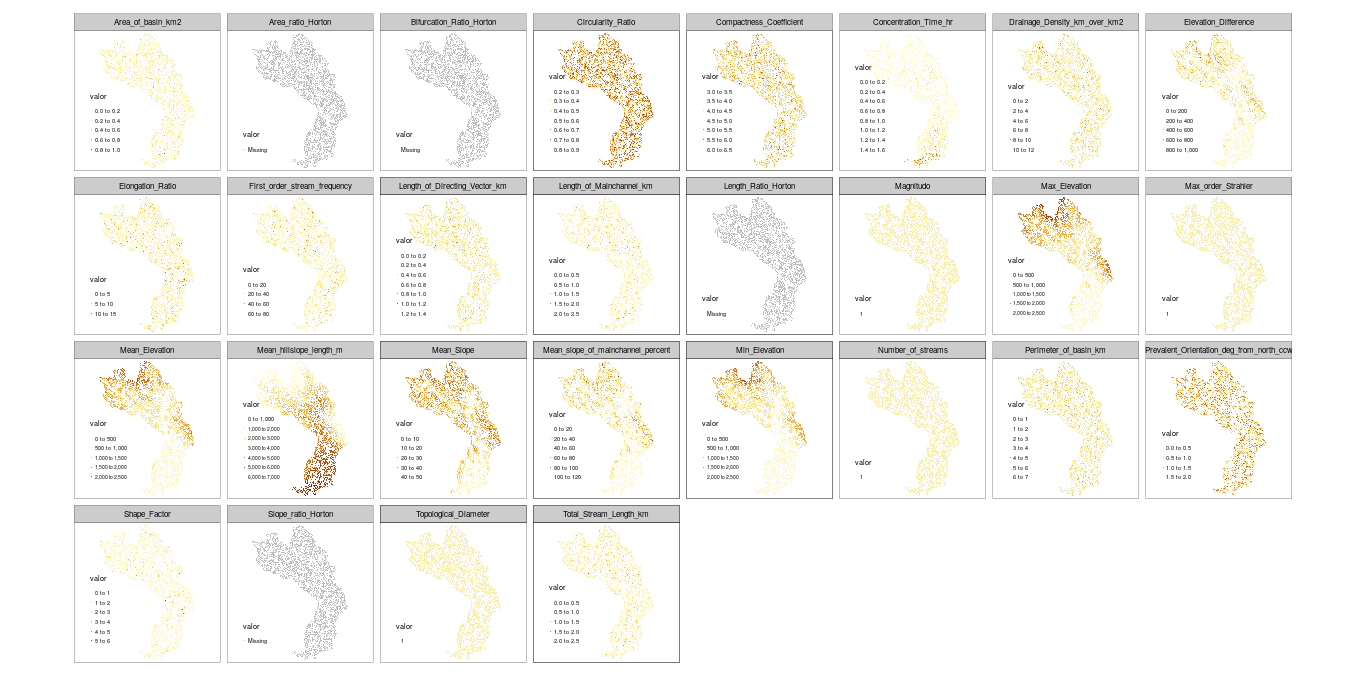
\includegraphics{Imagenes/Var_Sthraler.png}
\caption{Selección Variable Sthraler}
\end{figure}

Unión espacial de los datos

\begin{verbatim}
## Simple feature collection with 3027 features and 12 fields
## geometry type:  POLYGON
## dimension:      XY
## bbox:           xmin: 317400 ymin: 2019180 xmax: 352260 ymax: 2067690
## epsg (SRID):    32619
## proj4string:    +proj=utm +zone=19 +datum=WGS84 +units=m +no_defs
## First 10 features:
##        fid cat value label       DD        SF        ER     TS    MS
## 1  3.0e+09   2     1       2.189137 0.4974215 1.1522986 0.5194 26.44
## 2  4.0e+09   3     3       1.317045 1.5193957 6.7526210 0.0849 31.26
## 3  5.0e+09   7     2       5.021898 0.2158705 0.8774590 0.3870 24.12
## 4  6.0e+09  11    18       3.348350 0.3116489 0.7588246 0.7191 27.12
## 5  7.0e+09   8     8       1.323741 0.9530676 3.2504695 0.1449 36.98
## 6  8.0e+09   9     4       5.407681 0.2022916 0.7547642 0.4946 23.41
## 7  9.0e+09  12    10       1.707515 0.6384885 1.5645024 0.3621 34.67
## 8  1.0e+10  14     9       1.776552 0.7101480 2.8058127 0.1449 37.30
## 9  1.1e+10  15    14       1.017378 1.2400654 3.7077166 0.1449 37.36
## 10 1.2e+10  10    13       1.376470 0.8268738 2.2012308 0.2473 30.57
##        logDD        x       y                       geometry
## 1  0.7835072 334063.9 2067449 POLYGON ((334500 2067660, 3...
## 2  0.2753904 334582.9 2067514 POLYGON ((334500 2067390, 3...
## 3  1.6138079 334172.4 2067265 POLYGON ((334440 2067330, 3...
## 4  1.2084677 334366.4 2066754 POLYGON ((333840 2067180, 3...
## 5  0.2804618 333919.7 2066981 POLYGON ((333750 2067240, 3...
## 6  1.6878203 334365.9 2067039 POLYGON ((334380 2067240, 3...
## 7  0.5350394 333028.9 2066963 POLYGON ((332640 2067120, 3...
## 8  0.5746743 333771.9 2066901 POLYGON ((333540 2067090, 3...
## 9  0.0172283 333384.3 2066840 POLYGON ((333330 2067090, 3...
## 10 0.3195221 332580.6 2066931 POLYGON ((332280 2067000, 3...
\end{verbatim}

Unión espacial de los datos

\includegraphics{proyecto_files/figure-latex/unnamed-chunk-4-1.pdf}

\begin{verbatim}
##                                          Area_of_basin_km2
## Area_of_basin_km2                             1.0000000000
## Perimeter_of_basin_km                         0.9544758340
## Max_Elevation                                 0.1085164535
## Min_Elevation                                -0.0037333059
## Elevation_Difference                          0.4687069509
## Mean_Elevation                                0.0527159463
## Mean_Slope                                    0.0116722827
## Length_of_Directing_Vector_km                 0.8821719458
## Prevalent_Orientation_deg_from_north_ccw      0.0133206854
## Compactness_Coefficient                       0.3026490133
## Circularity_Ratio                            -0.2885703636
## Elongation_Ratio                             -0.4201325677
## Shape_Factor                                 -0.1774118107
## Concentration_Time_hr                         0.3376141894
## Length_of_Mainchannel_km                      0.8868782573
## Mean_slope_of_mainchannel_percent            -0.0000623078
## Mean_hillslope_length_m                      -0.0868302019
## Total_Stream_Length_km                        0.8866554994
## First_order_stream_frequency                 -0.6765432843
## Drainage_Density_km_over_km2                 -0.0999198137
##                                          Perimeter_of_basin_km
## Area_of_basin_km2                                  0.954475834
## Perimeter_of_basin_km                              1.000000000
## Max_Elevation                                      0.126072976
## Min_Elevation                                      0.003374361
## Elevation_Difference                               0.517032317
## Mean_Elevation                                     0.064253895
## Mean_Slope                                         0.007432527
## Length_of_Directing_Vector_km                      0.941048386
## Prevalent_Orientation_deg_from_north_ccw           0.005013254
## Compactness_Coefficient                            0.524072883
## Circularity_Ratio                                 -0.505511388
## Elongation_Ratio                                  -0.465434321
## Shape_Factor                                      -0.222059361
## Concentration_Time_hr                              0.323183639
## Length_of_Mainchannel_km                           0.912566038
## Mean_slope_of_mainchannel_percent                  0.011612370
## Mean_hillslope_length_m                           -0.097546277
## Total_Stream_Length_km                             0.912065876
## First_order_stream_frequency                      -0.729729329
## Drainage_Density_km_over_km2                      -0.037858082
##                                          Max_Elevation Min_Elevation
## Area_of_basin_km2                          0.108516454  -0.003733306
## Perimeter_of_basin_km                      0.126072976   0.003374361
## Max_Elevation                              1.000000000   0.979845711
## Min_Elevation                              0.979845711   1.000000000
## Elevation_Difference                       0.701703589   0.545241433
## Mean_Elevation                             0.994679678   0.994064553
## Mean_Slope                                 0.750349000   0.669770309
## Length_of_Directing_Vector_km              0.152748940   0.026447839
## Prevalent_Orientation_deg_from_north_ccw   0.008534377   0.011223559
## Compactness_Coefficient                    0.097747484   0.026836115
## Circularity_Ratio                         -0.100979358  -0.030532368
## Elongation_Ratio                          -0.034917788   0.019213707
## Shape_Factor                               0.014803339   0.034733040
## Concentration_Time_hr                     -0.522952456  -0.499344963
## Length_of_Mainchannel_km                   0.050522470  -0.053047221
## Mean_slope_of_mainchannel_percent          0.682330464   0.612424193
## Mean_hillslope_length_m                   -0.976100493  -0.966412179
## Total_Stream_Length_km                     0.050305343  -0.053392624
## First_order_stream_frequency              -0.104632503  -0.004045040
## Drainage_Density_km_over_km2              -0.080209378  -0.063762484
##                                          Elevation_Difference
## Area_of_basin_km2                                 0.468706951
## Perimeter_of_basin_km                             0.517032317
## Max_Elevation                                     0.701703589
## Min_Elevation                                     0.545241433
## Elevation_Difference                              1.000000000
## Mean_Elevation                                    0.628662419
## Mean_Slope                                        0.759984277
## Length_of_Directing_Vector_km                     0.546682345
## Prevalent_Orientation_deg_from_north_ccw         -0.004216387
## Compactness_Coefficient                           0.314482816
## Circularity_Ratio                                -0.314862013
## Elongation_Ratio                                 -0.215062688
## Shape_Factor                                     -0.061759832
## Concentration_Time_hr                            -0.413566386
## Length_of_Mainchannel_km                          0.401222022
## Mean_slope_of_mainchannel_percent                 0.679079570
## Mean_hillslope_length_m                          -0.649322231
## Total_Stream_Length_km                            0.401542793
## First_order_stream_frequency                     -0.424664856
## Drainage_Density_km_over_km2                     -0.109178547
##                                          Mean_Elevation   Mean_Slope
## Area_of_basin_km2                           0.052715946  0.011672283
## Perimeter_of_basin_km                       0.064253895  0.007432527
## Max_Elevation                               0.994679678  0.750349000
## Min_Elevation                               0.994064553  0.669770309
## Elevation_Difference                        0.628662419  0.759984277
## Mean_Elevation                              1.000000000  0.717902080
## Mean_Slope                                  0.717902080  1.000000000
## Length_of_Directing_Vector_km               0.091595925  0.043152236
## Prevalent_Orientation_deg_from_north_ccw    0.008888368 -0.036953776
## Compactness_Coefficient                     0.058377050 -0.039121906
## Circularity_Ratio                          -0.061951571  0.031780506
## Elongation_Ratio                           -0.006958558  0.066886548
## Shape_Factor                                0.026491708  0.109470202
## Concentration_Time_hr                      -0.513112068 -0.688395113
## Length_of_Mainchannel_km                   -0.001812884 -0.074929355
## Mean_slope_of_mainchannel_percent           0.660296508  0.791702711
## Mean_hillslope_length_m                    -0.976432501 -0.725848165
## Total_Stream_Length_km                     -0.002122928 -0.075037094
## First_order_stream_frequency               -0.056487200 -0.070666731
## Drainage_Density_km_over_km2               -0.074394042 -0.178183177
##                                          Length_of_Directing_Vector_km
## Area_of_basin_km2                                           0.88217195
## Perimeter_of_basin_km                                       0.94104839
## Max_Elevation                                               0.15274894
## Min_Elevation                                               0.02644784
## Elevation_Difference                                        0.54668234
## Mean_Elevation                                              0.09159593
## Mean_Slope                                                  0.04315224
## Length_of_Directing_Vector_km                               1.00000000
## Prevalent_Orientation_deg_from_north_ccw                    0.00272695
## Compactness_Coefficient                                     0.54755642
## Circularity_Ratio                                          -0.53162055
## Elongation_Ratio                                           -0.47271463
## Shape_Factor                                               -0.26333595
## Concentration_Time_hr                                       0.26489121
## Length_of_Mainchannel_km                                    0.90154020
## Mean_slope_of_mainchannel_percent                           0.04130672
## Mean_hillslope_length_m                                    -0.12424888
## Total_Stream_Length_km                                      0.90087307
## First_order_stream_frequency                               -0.66625572
## Drainage_Density_km_over_km2                                0.05523891
##                                          Prevalent_Orientation_deg_from_north_ccw
## Area_of_basin_km2                                                     0.013320685
## Perimeter_of_basin_km                                                 0.005013254
## Max_Elevation                                                         0.008534377
## Min_Elevation                                                         0.011223559
## Elevation_Difference                                                 -0.004216387
## Mean_Elevation                                                        0.008888368
## Mean_Slope                                                           -0.036953776
## Length_of_Directing_Vector_km                                         0.002726950
## Prevalent_Orientation_deg_from_north_ccw                              1.000000000
## Compactness_Coefficient                                              -0.038263247
## Circularity_Ratio                                                     0.047959520
## Elongation_Ratio                                                      0.020435968
## Shape_Factor                                                          0.028979551
## Concentration_Time_hr                                                 0.045817442
## Length_of_Mainchannel_km                                             -0.014559540
## Mean_slope_of_mainchannel_percent                                    -0.041954144
## Mean_hillslope_length_m                                              -0.006101928
## Total_Stream_Length_km                                               -0.014834648
## First_order_stream_frequency                                         -0.025730089
## Drainage_Density_km_over_km2                                         -0.062373016
##                                          Compactness_Coefficient
## Area_of_basin_km2                                    0.302649013
## Perimeter_of_basin_km                                0.524072883
## Max_Elevation                                        0.097747484
## Min_Elevation                                        0.026836115
## Elevation_Difference                                 0.314482816
## Mean_Elevation                                       0.058377050
## Mean_Slope                                          -0.039121906
## Length_of_Directing_Vector_km                        0.547556416
## Prevalent_Orientation_deg_from_north_ccw            -0.038263247
## Compactness_Coefficient                              1.000000000
## Circularity_Ratio                                   -0.982893198
## Elongation_Ratio                                    -0.274815245
## Shape_Factor                                        -0.253076546
## Concentration_Time_hr                                0.084829477
## Length_of_Mainchannel_km                             0.477967483
## Mean_slope_of_mainchannel_percent                    0.002602623
## Mean_hillslope_length_m                             -0.074702534
## Total_Stream_Length_km                               0.476467186
## First_order_stream_frequency                        -0.161420996
## Drainage_Density_km_over_km2                         0.310395399
##                                          Circularity_Ratio
## Area_of_basin_km2                             -0.288570364
## Perimeter_of_basin_km                         -0.505511388
## Max_Elevation                                 -0.100979358
## Min_Elevation                                 -0.030532368
## Elevation_Difference                          -0.314862013
## Mean_Elevation                                -0.061951571
## Mean_Slope                                     0.031780506
## Length_of_Directing_Vector_km                 -0.531620546
## Prevalent_Orientation_deg_from_north_ccw       0.047959520
## Compactness_Coefficient                       -0.982893198
## Circularity_Ratio                              1.000000000
## Elongation_Ratio                               0.289513381
## Shape_Factor                                   0.265974071
## Concentration_Time_hr                         -0.074379454
## Length_of_Mainchannel_km                      -0.459171337
## Mean_slope_of_mainchannel_percent             -0.006744063
## Mean_hillslope_length_m                        0.078708721
## Total_Stream_Length_km                        -0.457493385
## First_order_stream_frequency                   0.168318540
## Drainage_Density_km_over_km2                  -0.309107811
##                                          Elongation_Ratio Shape_Factor
## Area_of_basin_km2                            -0.420132568  -0.17741181
## Perimeter_of_basin_km                        -0.465434321  -0.22205936
## Max_Elevation                                -0.034917788   0.01480334
## Min_Elevation                                 0.019213707   0.03473304
## Elevation_Difference                         -0.215062688  -0.06175983
## Mean_Elevation                               -0.006958558   0.02649171
## Mean_Slope                                    0.066886548   0.10947020
## Length_of_Directing_Vector_km                -0.472714634  -0.26333595
## Prevalent_Orientation_deg_from_north_ccw      0.020435968   0.02897955
## Compactness_Coefficient                      -0.274815245  -0.25307655
## Circularity_Ratio                             0.289513381   0.26597407
## Elongation_Ratio                              1.000000000   0.92166632
## Shape_Factor                                  0.921666316   1.00000000
## Concentration_Time_hr                        -0.244967627  -0.18437450
## Length_of_Mainchannel_km                     -0.595756838  -0.43862982
## Mean_slope_of_mainchannel_percent             0.013563039   0.05012741
## Mean_hillslope_length_m                       0.054309895   0.02193559
## Total_Stream_Length_km                       -0.594894045  -0.43777825
## First_order_stream_frequency                  0.370979755   0.06989293
## Drainage_Density_km_over_km2                 -0.546157778  -0.66918169
##                                          Concentration_Time_hr
## Area_of_basin_km2                                   0.33761419
## Perimeter_of_basin_km                               0.32318364
## Max_Elevation                                      -0.52295246
## Min_Elevation                                      -0.49934496
## Elevation_Difference                               -0.41356639
## Mean_Elevation                                     -0.51311207
## Mean_Slope                                         -0.68839511
## Length_of_Directing_Vector_km                       0.26489121
## Prevalent_Orientation_deg_from_north_ccw            0.04581744
## Compactness_Coefficient                             0.08482948
## Circularity_Ratio                                  -0.07437945
## Elongation_Ratio                                   -0.24496763
## Shape_Factor                                       -0.18437450
## Concentration_Time_hr                               1.00000000
## Length_of_Mainchannel_km                            0.37973458
## Mean_slope_of_mainchannel_percent                  -0.54157779
## Mean_hillslope_length_m                             0.53319066
## Total_Stream_Length_km                              0.37928755
## First_order_stream_frequency                       -0.22050640
## Drainage_Density_km_over_km2                        0.12574975
##                                          Length_of_Mainchannel_km
## Area_of_basin_km2                                     0.886878257
## Perimeter_of_basin_km                                 0.912566038
## Max_Elevation                                         0.050522470
## Min_Elevation                                        -0.053047221
## Elevation_Difference                                  0.401222022
## Mean_Elevation                                       -0.001812884
## Mean_Slope                                           -0.074929355
## Length_of_Directing_Vector_km                         0.901540197
## Prevalent_Orientation_deg_from_north_ccw             -0.014559540
## Compactness_Coefficient                               0.477967483
## Circularity_Ratio                                    -0.459171337
## Elongation_Ratio                                     -0.595756838
## Shape_Factor                                         -0.438629821
## Concentration_Time_hr                                 0.379734584
## Length_of_Mainchannel_km                              1.000000000
## Mean_slope_of_mainchannel_percent                    -0.048088478
## Mean_hillslope_length_m                              -0.053644883
## Total_Stream_Length_km                                0.999712141
## First_order_stream_frequency                         -0.577404672
## Drainage_Density_km_over_km2                          0.273665370
##                                          Mean_slope_of_mainchannel_percent
## Area_of_basin_km2                                            -0.0000623078
## Perimeter_of_basin_km                                         0.0116123695
## Max_Elevation                                                 0.6823304637
## Min_Elevation                                                 0.6124241933
## Elevation_Difference                                          0.6790795702
## Mean_Elevation                                                0.6602965081
## Mean_Slope                                                    0.7917027108
## Length_of_Directing_Vector_km                                 0.0413067240
## Prevalent_Orientation_deg_from_north_ccw                     -0.0419541444
## Compactness_Coefficient                                       0.0026026227
## Circularity_Ratio                                            -0.0067440632
## Elongation_Ratio                                              0.0135630387
## Shape_Factor                                                  0.0501274147
## Concentration_Time_hr                                        -0.5415777885
## Length_of_Mainchannel_km                                     -0.0480884780
## Mean_slope_of_mainchannel_percent                             1.0000000000
## Mean_hillslope_length_m                                      -0.6681192684
## Total_Stream_Length_km                                       -0.0474631511
## First_order_stream_frequency                                 -0.0557148988
## Drainage_Density_km_over_km2                                 -0.0801406065
##                                          Mean_hillslope_length_m
## Area_of_basin_km2                                   -0.086830202
## Perimeter_of_basin_km                               -0.097546277
## Max_Elevation                                       -0.976100493
## Min_Elevation                                       -0.966412179
## Elevation_Difference                                -0.649322231
## Mean_Elevation                                      -0.976432501
## Mean_Slope                                          -0.725848165
## Length_of_Directing_Vector_km                       -0.124248878
## Prevalent_Orientation_deg_from_north_ccw            -0.006101928
## Compactness_Coefficient                             -0.074702534
## Circularity_Ratio                                    0.078708721
## Elongation_Ratio                                     0.054309895
## Shape_Factor                                         0.021935590
## Concentration_Time_hr                                0.533190662
## Length_of_Mainchannel_km                            -0.053644883
## Mean_slope_of_mainchannel_percent                   -0.668119268
## Mean_hillslope_length_m                              1.000000000
## Total_Stream_Length_km                              -0.053467451
## First_order_stream_frequency                         0.068526699
## Drainage_Density_km_over_km2                         0.027552614
##                                          Total_Stream_Length_km
## Area_of_basin_km2                                   0.886655499
## Perimeter_of_basin_km                               0.912065876
## Max_Elevation                                       0.050305343
## Min_Elevation                                      -0.053392624
## Elevation_Difference                                0.401542793
## Mean_Elevation                                     -0.002122928
## Mean_Slope                                         -0.075037094
## Length_of_Directing_Vector_km                       0.900873075
## Prevalent_Orientation_deg_from_north_ccw           -0.014834648
## Compactness_Coefficient                             0.476467186
## Circularity_Ratio                                  -0.457493385
## Elongation_Ratio                                   -0.594894045
## Shape_Factor                                       -0.437778253
## Concentration_Time_hr                               0.379287551
## Length_of_Mainchannel_km                            0.999712141
## Mean_slope_of_mainchannel_percent                  -0.047463151
## Mean_hillslope_length_m                            -0.053467451
## Total_Stream_Length_km                              1.000000000
## First_order_stream_frequency                       -0.577169211
## Drainage_Density_km_over_km2                        0.274631240
##                                          First_order_stream_frequency
## Area_of_basin_km2                                         -0.67654328
## Perimeter_of_basin_km                                     -0.72972933
## Max_Elevation                                             -0.10463250
## Min_Elevation                                             -0.00404504
## Elevation_Difference                                      -0.42466486
## Mean_Elevation                                            -0.05648720
## Mean_Slope                                                -0.07066673
## Length_of_Directing_Vector_km                             -0.66625572
## Prevalent_Orientation_deg_from_north_ccw                  -0.02573009
## Compactness_Coefficient                                   -0.16142100
## Circularity_Ratio                                          0.16831854
## Elongation_Ratio                                           0.37097976
## Shape_Factor                                               0.06989293
## Concentration_Time_hr                                     -0.22050640
## Length_of_Mainchannel_km                                  -0.57740467
## Mean_slope_of_mainchannel_percent                         -0.05571490
## Mean_hillslope_length_m                                    0.06852670
## Total_Stream_Length_km                                    -0.57716921
## First_order_stream_frequency                               1.00000000
## Drainage_Density_km_over_km2                               0.33133675
##                                          Drainage_Density_km_over_km2
## Area_of_basin_km2                                         -0.09991981
## Perimeter_of_basin_km                                     -0.03785808
## Max_Elevation                                             -0.08020938
## Min_Elevation                                             -0.06376248
## Elevation_Difference                                      -0.10917855
## Mean_Elevation                                            -0.07439404
## Mean_Slope                                                -0.17818318
## Length_of_Directing_Vector_km                              0.05523891
## Prevalent_Orientation_deg_from_north_ccw                  -0.06237302
## Compactness_Coefficient                                    0.31039540
## Circularity_Ratio                                         -0.30910781
## Elongation_Ratio                                          -0.54615778
## Shape_Factor                                              -0.66918169
## Concentration_Time_hr                                      0.12574975
## Length_of_Mainchannel_km                                   0.27366537
## Mean_slope_of_mainchannel_percent                         -0.08014061
## Mean_hillslope_length_m                                    0.02755261
## Total_Stream_Length_km                                     0.27463124
## First_order_stream_frequency                               0.33133675
## Drainage_Density_km_over_km2                               1.00000000
\end{verbatim}

El análisis de correlación entre la variable dependiente seleccionada
(Densidad de Drenaje) y las demás sometidas a prueba, resultaron con
índice mayor a 0.5 factor de forma (-0.669485228) y ratio de elongación
(-0.545994239). Para dar mayor robustez al modelo que se diseñó, se
incorporaron las variables: pendiente promedio (-0.176066777) y longitud
total del curso principal medido en km (0.274832295).

Comprobación del supuesto de distribución normal de las observaciones de
las variables analizadas

La comprobación del supuesto de normalidad se hizo mediante el gráfico
cuantilar de las variables donde se incluyó el ajuste logarítmico de la
variable dependiente a consecuencia del sesgo evidenciado ya que se
puede tolerar la no distribución normal de las independientes, no asi en
la dependiente.

\begin{figure}
\centering
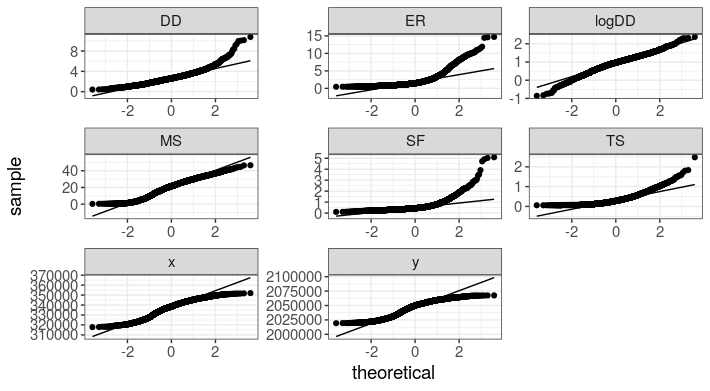
\includegraphics{Imagenes/pruebanormshapiro.png}
\caption{Estadistica cuantilar variables utilizadas}
\end{figure}

Se asume como válido el supuesto de normalidad de los datos tanto en el
diagrama cuantilar normal en el cual se muestra un relativo acercamiento
de los puntos a una forma de la recta que representan las observaciones
de cada una de las variables analizadas, como los indicadores numéricos
de la prueba de Shapiro-Wilk con ``p'' menores a 0.05, indicando
significancia y que se cumple el supuesto de distribución normal de los
datos de las variables analizadas.

Comprobación de supuesto de autocorrelación de la variable dependiente
transformada (I de Moran Global).

\begin{figure}
\centering
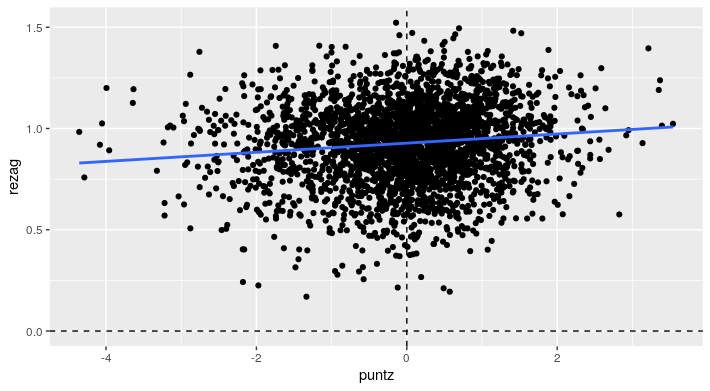
\includegraphics{Imagenes/DiagDisperMoran.png}
\caption{Diagrama Dispersion G.Moran}
\end{figure}

Visualización porcentual de la dispersión de la Variable seleccionada
Densidad de Drenage ajustada logarítmicamente en cuatro cuadrantes

\begin{figure}
\centering
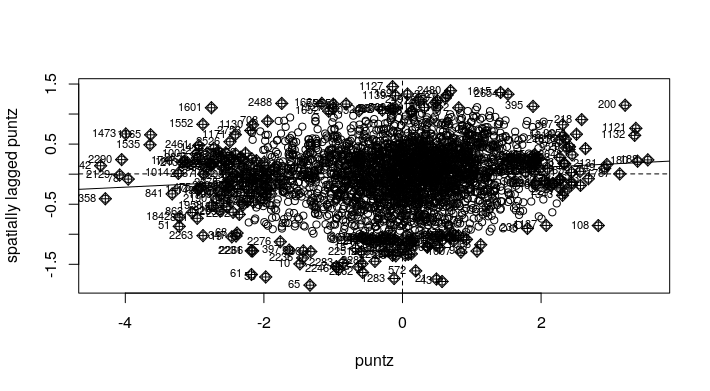
\includegraphics{Imagenes/MoranplotpesoW.png}
\caption{Diagrama dispersion Moran PesoW}
\end{figure}

Se rechaza preliminarmente la hipótesis nula la cual sostiene que NO hay
autocorrelación espacial dado un valor de ``p''\textless{} 0.05
(6.07e-05) y se acepta la hipótesis alternativa de que existe
autocorrelación espacial global.

\begin{figure}
\centering
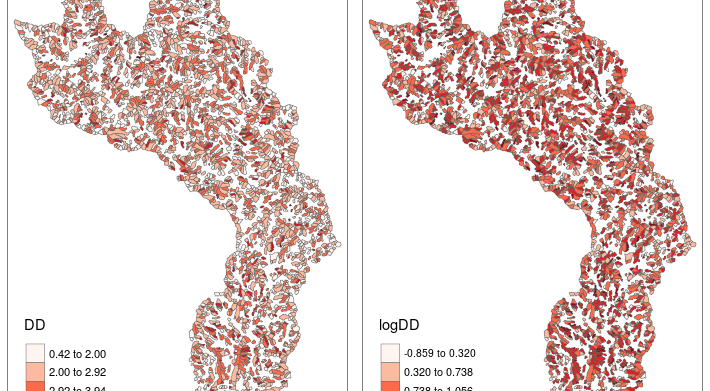
\includegraphics{Imagenes/p2DDlogDD.png}
\caption{Variable dependiente original y ajustada log.}
\end{figure}

Evaluación de la autocorrelación espacial local de la variable
dependiente transformada

\begin{figure}
\centering
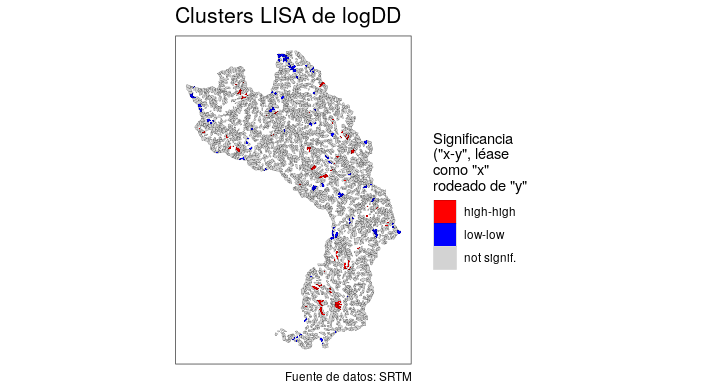
\includegraphics{Imagenes/ClusterLisalogDD.png}
\caption{Lisa Cluster Variable Dependiente Transformada LogDD}
\end{figure}

La aparición de parches rojos y azules indican la existencia de
autocorrelación local. Los parches rojos traducen hotspots o altos
valores de correlación. Los parches azules traducen coldspots e indican
autocorrelación con valores bajos. Finalmente, los valores grises
indican ausencia de correlación local.

Análisis de vecindad por contigüidad (vecxcont)

Resultaron 3027 regiones ya que cada observación en este caso funge como
una unidad espacial independiente. La prueba de peso homogéneo de
vecindad arrojó 5760 conexiones distintas de cero con un promedio de
conexiones de 1.901618 para un valor porcentual de 6.28\%, dos regiones
con 9 conexiones y 695 regiones sin conexión alguna.

Análisis de Vecindad por cantidad de los 5 vecinos más cercanos Los
valores de la data completa y la de los 5 vecinos más cercanos ya que
cada observación corresponde a una unidad espacial, es decir,
absolutamente todas las observaciones son vecinos entre si (In
knearneigh(coords, k = 5) : knearneigh: identical points found).

Análisis de Vecindad por peso de observaciones vecinas en Varselpol3 Por
tratarse de un espacio geográfico limitado cuyas unidades espaciales
(microcuencas) corresponden a las mismas observaciones puntuales, los
valores de conexiones y vecindades no difieren mucho en las diferentes
combinaciones de vecindad examinadas. En este caso el número de regiones
sigue siendo 3027. Las conexiones diferentes de cero son 15145, el
porcentaje de conexiones no cero es 16.5\% y el promedio de conexiones
es de 5.

Modelización

Visualización porcentual de la dispersión de la Variable seleccionada
Densidad de Drenaje ajustada logarítmicamente en cuatro cuadrantes

\begin{figure}
\centering
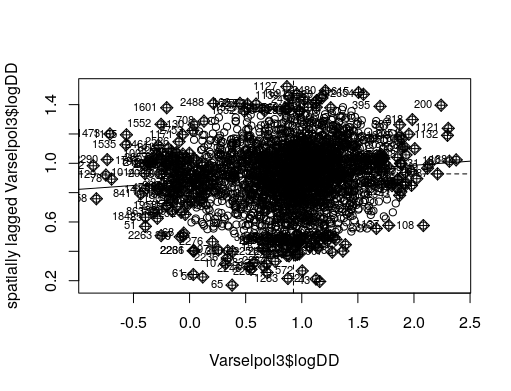
\includegraphics{Imagenes/moranValselpol3logDD.png}
\caption{Variable seleccionada Densidad de drenaje log.}
\end{figure}

Comprobación del Supuesto de Autocorrelación mediante la Prueba de Moran
Global:

\begin{figure}
\centering
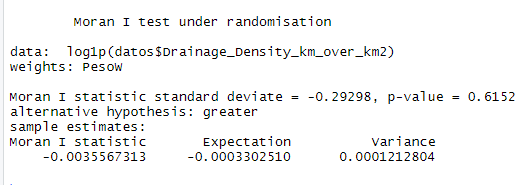
\includegraphics{Imagenes/gmoranW.png}
\caption{Comprobacion supuesto autorrelacion}
\end{figure}

El valor de ``p'' es mayor a 0.05 (valor comunmente establecido), se
acepta la hipotesis nula ``No hay autocorrelación espacial global'' con
sus vecinos en la variable dependiente en su versión original. Aunque el
sistema de cuenta de la aceptación de la misma (alternative hyphotesis:
greater).

\begin{figure}
\centering
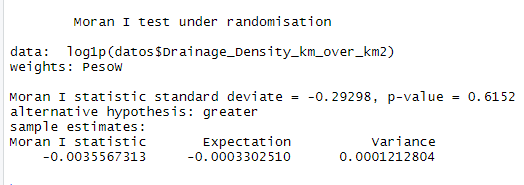
\includegraphics{Imagenes/gmoranWB.png}
\caption{Supuesto correlacion variable}
\end{figure}

En el caso de la prueba de los supuestos de autocorrelación de la
variable tanto por contigüidad como por peso coinciden por la misma
causa que en el análisis de vecindad en entidades poligonales, las
unidades espaciales (microcuencas) son los mismos puntos de observación,
es decir, tenemos tantos modelos como puntos de observación en el
análisis.

\begin{figure}
\centering
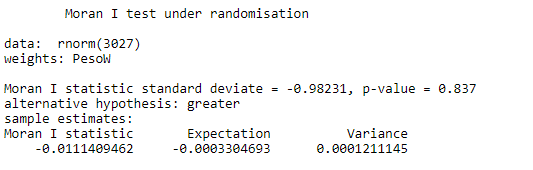
\includegraphics{Imagenes/gmoranWBhip.png}
\caption{Hipotesis alternativa}
\end{figure}

El valor de ``p'' es mayor a 0.05 (valor comunmente establecido), se
acepta la hipotesis nula ``No hay autocorrelación espacial global'' con
sus vecinos respecto a la variable porcentual ajustada por logaritmo.
Aunque el sistema de cuenta de la aceptación de la misma (alternative
hyphotesis: greater).

\begin{figure}
\centering
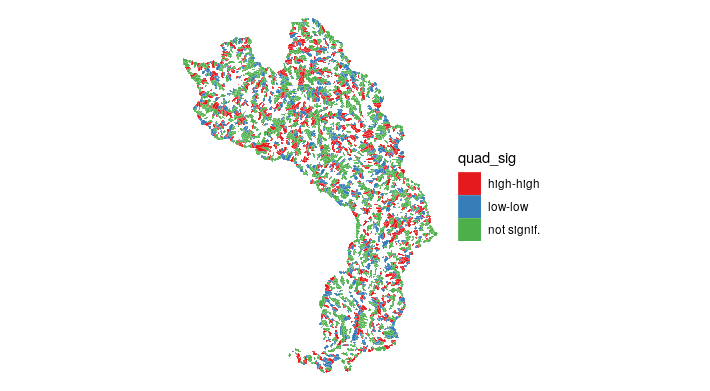
\includegraphics{Imagenes/autesplocal.png}
\caption{Correlación local Variable Log.}
\end{figure}

Comprobación del supuesto de normalidad (shapiro-wilk)

data: Varselpctlog\$logDD\_PCT W = 0.33291, p-value \textless{} 2.2e-16

El valor de ``p'' es menor a 0.05 (2.2e-16), se rechaza la hipotesis
nula ``No hay distribución normal'' , en otras palabras se acepta la
hipotesis alternativa ``Existe distribución normal de las observaciones
de la variable analizada(Varselpctlog\$logDD\_PCT)''.

data: Varselpctlog\$logDD\_PCTLOG W = 0.36622, p-value \textless{}
2.2e-16

El valor de ``p'' es menor a 0.05 (2.2e-16), se rechaza la hipotesis
nula ``No hay distribución normal'' , en otras palabras se acepta la
hipotesis alternativa ``Existe distribución normal de las observaciones
de la variable analizada(Varselpctlog\$logDD\_PCTLOG)''. En sisntesis,
se cumple el supuesto de normalidad en ambas versiones de la variable
dependiente del modelo analizado.

Comprobación de supuesto de heterocedasticidad (prueba de Breusch-Pagan)

\begin{figure}
\centering
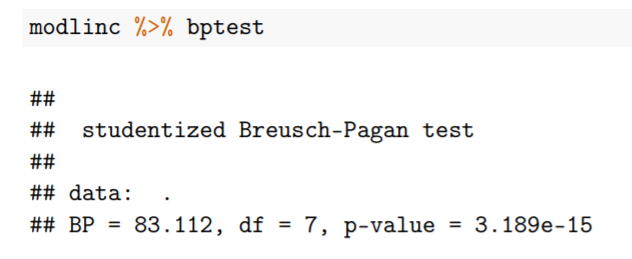
\includegraphics{Imagenes/breuschPagan.png}
\caption{Prueba de Breush-Pagan}
\end{figure}

El valor de ``p'' es menor a 0.05 (3.189e-15), se rechaza la hipotesis
nula ``No hay homocedasticidad'' , en otras palabras se acepta la
hipotesis alternativa ``Existe heterocedasticidad las observaciones de
las variables analizadas en el modelo lineal con la versión de ajuste
logaritmico de la variable dependiente.

Análisis del modelo lineal

\begin{figure}
\centering
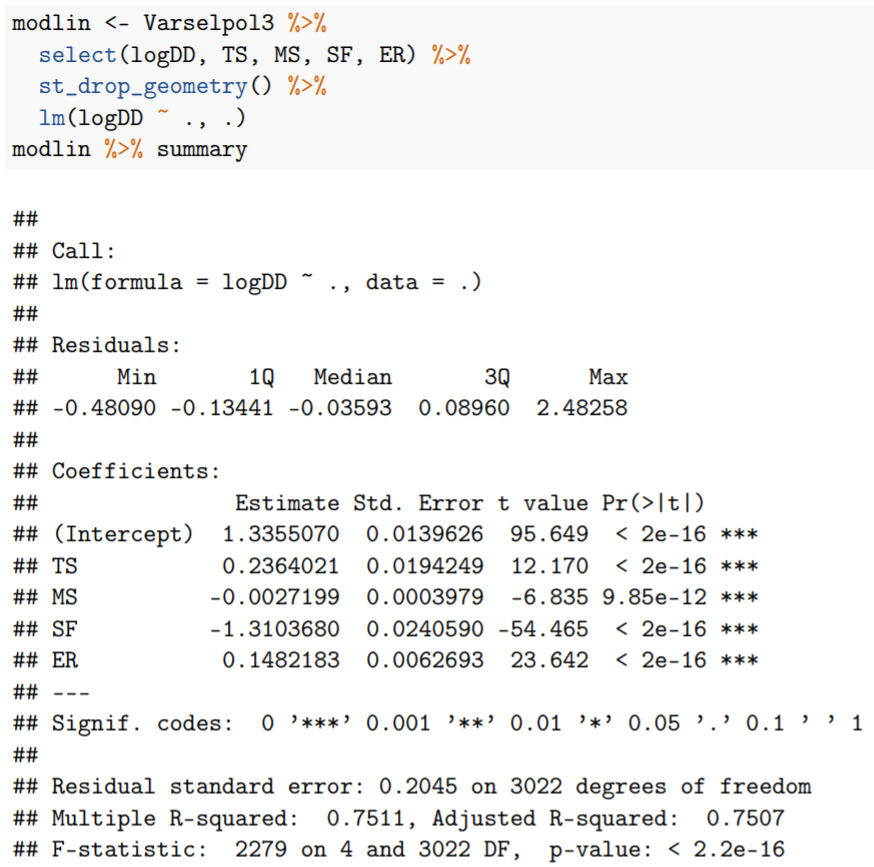
\includegraphics{Imagenes/modelolineal.png}
\caption{Análisis Modelo Lineal}
\end{figure}

Todos los coeficientes de las variables del modelo han resultado
signicativas (p\textless{}0.05) y el R cuadrado ajustado del modelo
indica que las variables independientes analizadas explican en un
75.07\% a la variable dependiente Dendidad de drenaje. Por otro lado, si
el valor de las independientes fuera cero, la variable dependiente
tomaria el valor 1.3355070 (intercepto).

Las demas pruebas correspondientes al mismo modelo lineal utilizando
versiones transformadas de las valiables(\% y Log e) resultaron no
significativos, es decir, las variables independientes analizadas no
logran explicar el comportamiento de la variable dependiente, en tanto,
no resultan útiles para la predicción de escenarios de la Densidad de
Drenaje de la cuenca del Rio Ocoa.

Análisis del modelo espacial autoregresivo (Variate Simultaneous
Autoregresive Model) No se profundizó este temario en el curso de la
asignatura

\begin{figure}
\centering
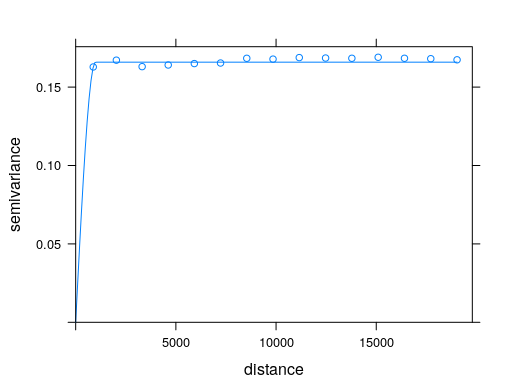
\includegraphics{Imagenes/semivarianzaMSph.png}
\caption{Variograma Modelo Sph}
\end{figure}

\begin{figure}
\centering
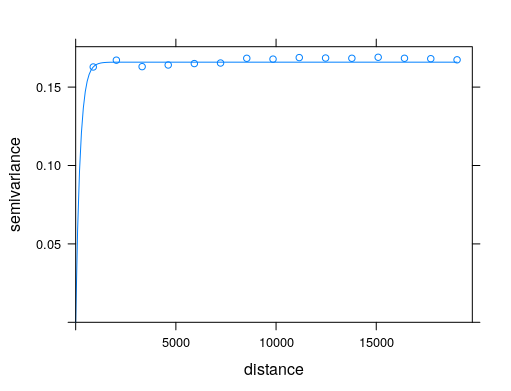
\includegraphics{Imagenes/SemivModelGau.png}
\caption{Variograma Modelo Gau}
\end{figure}

\begin{figure}
\centering
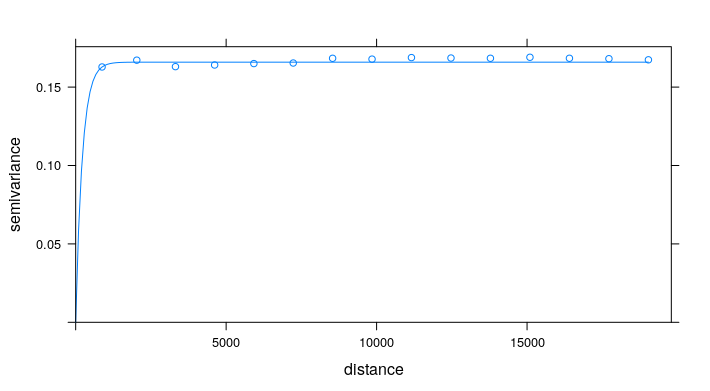
\includegraphics{Imagenes/semivmodExp.png}
\caption{Variograma Moded Exp}
\end{figure}

\begin{figure}
\centering
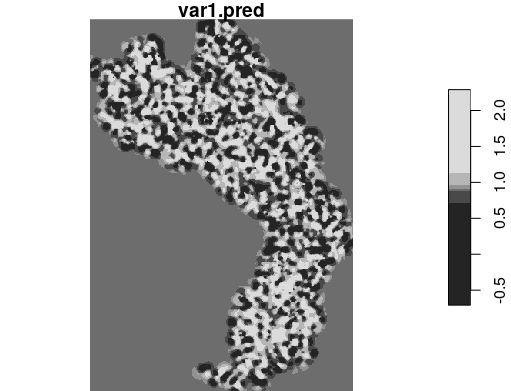
\includegraphics{Imagenes/kriging.var1.pred.png}
\caption{Kriging Ordinario}
\end{figure}

\ldots

\section{Información de soporte}\label{informaciuxf3n-de-soporte}

Material de Apoyo incluido en el repositorio de la maestría
Teledeteccion y Ciencias de la Informacion Geografica. Asesoría con el
profesor José Ramón Martínez.

\ldots

\section{\texorpdfstring{\emph{Script}
reproducible}{Script reproducible}}\label{script-reproducible}

\section{LIBRERIAS A UTILIZAR}\label{librerias-a-utilizar}

\begin{Shaded}
\begin{Highlighting}[]
\KeywordTok{library}\NormalTok{(sf)}
\KeywordTok{library}\NormalTok{(tidyverse)}
\KeywordTok{library}\NormalTok{(gstat)}
\KeywordTok{library}\NormalTok{(stars)}
\KeywordTok{library}\NormalTok{(tmap)}
\KeywordTok{library}\NormalTok{(ez)}
\KeywordTok{library}\NormalTok{(RColorBrewer)}
\KeywordTok{library}\NormalTok{ (sp)}
\KeywordTok{library}\NormalTok{(spdep) }
\KeywordTok{library}\NormalTok{(lmtest)}
\KeywordTok{library}\NormalTok{(spData)}
\KeywordTok{source}\NormalTok{(}\StringTok{'lisaclusters.R'}\NormalTok{)}
\end{Highlighting}
\end{Shaded}

IMPORTACION, ORGANIZACION DE DATOS E INTERPORABILIDAD

\section{Cargar datos de variables}\label{cargar-datos-de-variables}

\begin{Shaded}
\begin{Highlighting}[]
\NormalTok{(datos <-}\StringTok{ }\KeywordTok{st_read}\NormalTok{(}\StringTok{'paramsoutlet_orden1.gpkg'}\NormalTok{, }\DataTypeTok{crs =} \DecValTok{32619}\NormalTok{))}
\NormalTok{(datos <-}\StringTok{ }\NormalTok{datos }\OperatorTok\StringTok{ }\KeywordTok{st_difference}\NormalTok{())}
\NormalTok{(pol1 <-}\StringTok{ }\KeywordTok{st_read}\NormalTok{(}\DataTypeTok{dsn =} \StringTok{'r_stream_basins_1.geojson'}\NormalTok{, }\DataTypeTok{crs =} \DecValTok{32619}\NormalTok{))}
\NormalTok{pol2 <-}\StringTok{ }\KeywordTok{st_read}\NormalTok{(}\DataTypeTok{dsn =} \StringTok{'r_stream_basins_2.geojson'}\NormalTok{, }\DataTypeTok{crs =} \DecValTok{32619}\NormalTok{)}
\NormalTok{pol3 <-}\StringTok{ }\KeywordTok{st_read}\NormalTok{(}\DataTypeTok{dsn =} \StringTok{'r_stream_basins_3.geojson'}\NormalTok{, }\DataTypeTok{crs =} \DecValTok{32619}\NormalTok{)}
\NormalTok{pol4 <-}\StringTok{ }\KeywordTok{st_read}\NormalTok{(}\DataTypeTok{dsn =} \StringTok{'r_stream_basins_4.geojson'}\NormalTok{, }\DataTypeTok{crs =} \DecValTok{32619}\NormalTok{)}
\end{Highlighting}
\end{Shaded}

Orden de Red Cuencas 1, clasificacion de Strahler

\begin{Shaded}
\begin{Highlighting}[]
\NormalTok{datos }\OperatorTok\StringTok{ }\NormalTok{dplyr}\OperatorTok{::}\KeywordTok{filter}\NormalTok{(Max_order_Strahler}\OperatorTok{==}\DecValTok{1}\NormalTok{)}

\NormalTok{datos }\OperatorTok
\StringTok{  }\KeywordTok{select_if}\NormalTok{(is.numeric) }\OperatorTok
\StringTok{  }\KeywordTok{gather}\NormalTok{(variable, valor, }\OperatorTok{-}\NormalTok{geom) }\OperatorTok
\StringTok{  }\KeywordTok{st_drop_geometry}\NormalTok{() }\OperatorTok\StringTok{ }
\StringTok{  }\KeywordTok{group_by}\NormalTok{(variable) }\OperatorTok\StringTok{ }
\StringTok{  }\KeywordTok{summarise}\NormalTok{(}\DataTypeTok{m=}\KeywordTok{mean}\NormalTok{(valor, }\DataTypeTok{na.rm=}\NormalTok{T))}

\NormalTok{datos }\OperatorTok
\StringTok{  }\KeywordTok{select_if}\NormalTok{(is.numeric) }\OperatorTok
\StringTok{  }\KeywordTok{gather}\NormalTok{(variable, valor, }\OperatorTok{-}\NormalTok{geom) }\OperatorTok\StringTok{ }
\StringTok{  }\KeywordTok{tm_shape}\NormalTok{() }\OperatorTok{+}\StringTok{ }\KeywordTok{tm_dots}\NormalTok{(}\DataTypeTok{col =} \StringTok{'valor'}\NormalTok{) }\OperatorTok{+}\StringTok{ }\KeywordTok{tm_facets}\NormalTok{(}\DataTypeTok{by=}\StringTok{'variable'}\NormalTok{, }
    \DataTypeTok{free.coords =}\NormalTok{ F, }\DataTypeTok{free.scales =}\NormalTok{ T)}
\end{Highlighting}
\end{Shaded}

Tabla cols numericas, con varianza

\begin{Shaded}
\begin{Highlighting}[]
\NormalTok{datosnum <-}\StringTok{ }\NormalTok{datos }\OperatorTok
\StringTok{  }\KeywordTok{st_drop_geometry}\NormalTok{() }\OperatorTok\StringTok{ }
\StringTok{  }\KeywordTok{select_if}\NormalTok{(is.numeric) }\OperatorTok\StringTok{ }
\StringTok{  }\KeywordTok{select_if}\NormalTok{(}\OperatorTok{~}\StringTok{ }\KeywordTok{sum}\NormalTok{(}\OperatorTok{!}\KeywordTok{is.na}\NormalTok{(.))}\OperatorTok{>}\DecValTok{0}\NormalTok{) }\OperatorTok\StringTok{ }
\StringTok{  }\KeywordTok{select_if}\NormalTok{(}\ControlFlowTok{function}\NormalTok{(x) }\KeywordTok{var}\NormalTok{(x, }\DataTypeTok{na.rm=}\NormalTok{T)}\OperatorTok{!=}\DecValTok{0}\NormalTok{)}
\end{Highlighting}
\end{Shaded}

Evaluacion de correlacion entre las variables como criterio de seleccion

\begin{Shaded}
\begin{Highlighting}[]
\NormalTok{datosnum }\OperatorTok\StringTok{ }\KeywordTok{ezCor}\NormalTok{(}\DataTypeTok{r_size_lims =} \DecValTok{2}\OperatorTok{:}\DecValTok{3}\NormalTok{, }\DataTypeTok{label_size =} \DecValTok{2}\NormalTok{)}
\NormalTok{datosnum }\OperatorTok\StringTok{ }\NormalTok{cor}
\end{Highlighting}
\end{Shaded}

Union espacial de las variables seleccionadas

\begin{Shaded}
\begin{Highlighting}[]
\NormalTok{VARSEL <-}\StringTok{ }\NormalTok{datos }\OperatorTok\StringTok{ }
\StringTok{  }\NormalTok{dplyr}\OperatorTok{::}\KeywordTok{select}\NormalTok{(}
    \DataTypeTok{DD =}\NormalTok{ Drainage_Density_km_over_km2,}
    \DataTypeTok{SF =}\NormalTok{ Shape_Factor,}
    \DataTypeTok{ER =}\NormalTok{ Elongation_Ratio,}
    \DataTypeTok{TS =}\NormalTok{ Total_Stream_Length_km,}
    \DataTypeTok{MS =}\NormalTok{ Mean_Slope}
\NormalTok{  )}

\NormalTok{Varselpol1 <-}\StringTok{ }\NormalTok{pol1 }\OperatorTok\StringTok{ }\KeywordTok{st_join}\NormalTok{(}\DataTypeTok{left =}\NormalTok{ F, VARSEL)}
\NormalTok{Varselpol2 <-}\StringTok{ }\NormalTok{Varselpol1 }\OperatorTok\StringTok{ }
\StringTok{  }\KeywordTok{mutate}\NormalTok{(}\DataTypeTok{logDD =} \KeywordTok{log}\NormalTok{(DD))}
\end{Highlighting}
\end{Shaded}

Creación de objeto XY con atributos del objeto Varselpol2 mediante el
centroide de los polígonos

\begin{Shaded}
\begin{Highlighting}[]
\NormalTok{xy <-}\StringTok{ }\NormalTok{Varselpol2 }\OperatorTok
\StringTok{  }\KeywordTok{st_centroid}\NormalTok{() }\OperatorTok\StringTok{ }
\StringTok{  }\KeywordTok{mutate}\NormalTok{(}\DataTypeTok{x=}\KeywordTok{unlist}\NormalTok{(}\KeywordTok{map}\NormalTok{(geometry,}\DecValTok{1}\NormalTok{)),}
         \DataTypeTok{y=}\KeywordTok{unlist}\NormalTok{(}\KeywordTok{map}\NormalTok{(geometry,}\DecValTok{2}\NormalTok{))) }\OperatorTok\StringTok{ }
\StringTok{  }\KeywordTok{st_drop_geometry}\NormalTok{() }\OperatorTok\StringTok{ }
\StringTok{  }\KeywordTok{select}\NormalTok{(fid, x, y)}
\end{Highlighting}
\end{Shaded}

Creación del objeto Varselpol3 mediante unión de XY y Varselpol2

\begin{Shaded}
\begin{Highlighting}[]
\NormalTok{Varselpol3 <-}\StringTok{ }\NormalTok{Varselpol2 }\OperatorTok\StringTok{ }
\StringTok{  }\KeywordTok{inner_join}\NormalTok{(xy)}
\NormalTok{Varselpol3}
\end{Highlighting}
\end{Shaded}

VECINDAD. Analisis de vecindad por contiguidad

\begin{Shaded}
\begin{Highlighting}[]
\NormalTok{Varselpol3 <-}\StringTok{ }\NormalTok{Varselpol2 }\OperatorTok\StringTok{ }
\StringTok{  }\KeywordTok{inner_join}\NormalTok{(xy)}
\NormalTok{Varselpol3}
\end{Highlighting}
\end{Shaded}

Análisis de Vecindad por cantidad de los 5 vecinos más cercanos

\begin{Shaded}
\begin{Highlighting}[]
\NormalTok{Varselpol3.sp <-}\StringTok{ }\KeywordTok{as_Spatial}\NormalTok{(Varselpol3)}
\NormalTok{coords <-}\StringTok{ }\KeywordTok{coordinates}\NormalTok{(Varselpol3.sp)}
\NormalTok{VecxK <-}\StringTok{ }\KeywordTok{knn2nb}\NormalTok{(}\KeywordTok{knearneigh}\NormalTok{(coords, }\DataTypeTok{k=}\DecValTok{5}\NormalTok{))}
\end{Highlighting}
\end{Shaded}

Análisis de Vecindad por peso de observaciones vecinas en Varselpol3

\begin{Shaded}
\begin{Highlighting}[]
\NormalTok{PesoW <-}\StringTok{ }\KeywordTok{nb2listw}\NormalTok{(VecxK)}
\NormalTok{PesoW}

\NormalTok{PesowB <-}\StringTok{ }\KeywordTok{nb2listw}\NormalTok{(VecxK, }\DataTypeTok{style =} \StringTok{'B'}\NormalTok{)}
\NormalTok{PesowB}
\end{Highlighting}
\end{Shaded}

Análisis de Vecindad por peso de observaciones vecinas en la data
completa

\begin{Shaded}
\begin{Highlighting}[]
\NormalTok{datos <-}\StringTok{ }\NormalTok{datos }\OperatorTok\StringTok{ }\KeywordTok{st_difference}\NormalTok{()}
\NormalTok{coords <-}\StringTok{ }\KeywordTok{coordinates}\NormalTok{(}\KeywordTok{as_Spatial}\NormalTok{(datos))}
\NormalTok{nb <-}\StringTok{ }\KeywordTok{knn2nb}\NormalTok{(}\KeywordTok{knearneigh}\NormalTok{(coords, }\DataTypeTok{k =} \DecValTok{5}\NormalTok{))}
\KeywordTok{summary}\NormalTok{(nb)}
\end{Highlighting}
\end{Shaded}

ANALISIS ESDA

\begin{Shaded}
\begin{Highlighting}[]
\NormalTok{p1 <-}\StringTok{ }\KeywordTok{tm_shape}\NormalTok{(Varselpol3) }\OperatorTok{+}
\StringTok{  }\KeywordTok{tm_fill}\NormalTok{(}\DataTypeTok{col =} \StringTok{"DD"}\NormalTok{, }\DataTypeTok{style =} \StringTok{'jenks'}\NormalTok{, }\DataTypeTok{palette =} \KeywordTok{brewer.pal}\NormalTok{(}\DecValTok{9}\NormalTok{, }\DataTypeTok{name =} \StringTok{'Reds'}\NormalTok{)) }\OperatorTok{+}
\StringTok{  }\KeywordTok{tm_borders}\NormalTok{(}\DataTypeTok{lwd =} \FloatTok{0.5}\NormalTok{)}
\NormalTok{p1}

\NormalTok{p2 <-}\StringTok{ }\KeywordTok{tm_shape}\NormalTok{(Varselpol3) }\OperatorTok{+}
\StringTok{  }\KeywordTok{tm_fill}\NormalTok{(}\DataTypeTok{col =} \StringTok{"logDD"}\NormalTok{, }\DataTypeTok{style =} \StringTok{'jenks'}\NormalTok{,}
          \DataTypeTok{palette =} \KeywordTok{brewer.pal}\NormalTok{(}\DecValTok{9}\NormalTok{, }\DataTypeTok{name =} \StringTok{'Reds'}\NormalTok{), }\DataTypeTok{midpoint =} \OtherTok{NA}\NormalTok{) }\OperatorTok{+}
\StringTok{  }\KeywordTok{tm_borders}\NormalTok{(}\DataTypeTok{lwd =} \FloatTok{0.5}\NormalTok{)}
\KeywordTok{tmap_arrange}\NormalTok{(p1, p2)}

\NormalTok{Varselpol3 }\OperatorTok\StringTok{ }\KeywordTok{st_drop_geometry}\NormalTok{() }\OperatorTok
\StringTok{  }\KeywordTok{gather}\NormalTok{(variable, valor, }\OperatorTok{-}\NormalTok{(fid}\OperatorTok{:}\NormalTok{label)) }\OperatorTok
\StringTok{  }\KeywordTok{ggplot}\NormalTok{() }\OperatorTok{+}\StringTok{ }\KeywordTok{aes}\NormalTok{(}\DataTypeTok{sample=}\NormalTok{valor) }\OperatorTok{+}
\StringTok{  }\KeywordTok{stat_qq}\NormalTok{() }\OperatorTok{+}\StringTok{ }\KeywordTok{stat_qq_line}\NormalTok{() }\OperatorTok{+}\StringTok{ }\KeywordTok{theme_bw}\NormalTok{() }\OperatorTok{+}
\StringTok{  }\KeywordTok{theme}\NormalTok{(}\DataTypeTok{text =} \KeywordTok{element_text}\NormalTok{(}\DataTypeTok{size =} \DecValTok{14}\NormalTok{)) }\OperatorTok{+}
\StringTok{  }\KeywordTok{facet_wrap}\NormalTok{(}\OperatorTok{~}\NormalTok{variable, }\DataTypeTok{scales =} \StringTok{'free'}\NormalTok{)}

\NormalTok{Varselpol3 }\OperatorTok\StringTok{ }\KeywordTok{st_drop_geometry}\NormalTok{() }\OperatorTok
\StringTok{  }\KeywordTok{gather}\NormalTok{(variable, valor, }\OperatorTok{-}\NormalTok{(fid}\OperatorTok{:}\NormalTok{label)) }\OperatorTok\StringTok{ }\KeywordTok{group_by}\NormalTok{(variable) }\OperatorTok
\StringTok{  }\KeywordTok{summarise}\NormalTok{(}\DataTypeTok{prueba_normalidad=}\KeywordTok{shapiro.test}\NormalTok{(valor)}\OperatorTok{$}\NormalTok{p.value)}

\KeywordTok{lisamap}\NormalTok{(}\DataTypeTok{objesp =}\NormalTok{ Varselpol3,}
        \DataTypeTok{var =}\StringTok{'logDD'}\NormalTok{,}
        \DataTypeTok{pesos =}\NormalTok{ PesoW,}
        \DataTypeTok{tituloleyenda =} \StringTok{'Significancia}\CharTok{\textbackslash{}n}\StringTok{("x-y", léase}\CharTok{\textbackslash{}n}\StringTok{como "x"}\CharTok{\textbackslash{}n}\StringTok{rodeado de "y"'}\NormalTok{,}
        \DataTypeTok{leyenda =}\NormalTok{ T,}
        \DataTypeTok{anchuratitulo =} \DecValTok{1000}\NormalTok{,}
        \DataTypeTok{tamanotitulo =} \DecValTok{16}\NormalTok{,}
        \DataTypeTok{fuentedatos =} \StringTok{'SRTM'}\NormalTok{,}
        \DataTypeTok{titulomapa =} \KeywordTok{paste0}\NormalTok{(}\StringTok{'Clusters LISA de logDD'}\NormalTok{))}
\end{Highlighting}
\end{Shaded}

MODELIZACION

Variable seleccionada Densidad de Drenaje

\begin{Shaded}
\begin{Highlighting}[]
\NormalTok{Varselpctlog <-}\StringTok{ }\NormalTok{Varselpol3 }\OperatorTok\StringTok{ }\KeywordTok{mutate_each}\NormalTok{(}
  \KeywordTok{funs}\NormalTok{(}\DataTypeTok{PCT=}\KeywordTok{round}\NormalTok{(.}\OperatorTok{/}\NormalTok{DD,}\DecValTok{4}\NormalTok{)}\OperatorTok{*}\DecValTok{100}\NormalTok{,}
       \DataTypeTok{PCTLOG=}\KeywordTok{log}\NormalTok{(}\KeywordTok{round}\NormalTok{(.}\OperatorTok{/}\NormalTok{DD,}\DecValTok{4}\NormalTok{)}\OperatorTok{*}\DecValTok{100}\NormalTok{)),}
  \OperatorTok{-}\DecValTok{1}\NormalTok{, }\OperatorTok{-}\DecValTok{2}\NormalTok{, }\OperatorTok{-}\NormalTok{geometry, }\OperatorTok{-}\NormalTok{label)}

\NormalTok{Varselpctlog}
\end{Highlighting}
\end{Shaded}

Comprobando autocorrelación mediante la prueba moran global

\begin{Shaded}
\begin{Highlighting}[]
\KeywordTok{moran.plot}\NormalTok{(Varselpol3}\OperatorTok{$}\NormalTok{logDD, PesoW)}
\NormalTok{(gmoranw <-}\StringTok{ }\KeywordTok{moran.test}\NormalTok{(}\DataTypeTok{na.action =}\NormalTok{ na.exclude, }\DataTypeTok{zero.policy =}\NormalTok{ T,}
            \DataTypeTok{x =} \KeywordTok{log1p}\NormalTok{(datos}\OperatorTok{$}\NormalTok{Drainage_Density_km_over_km2), }\DataTypeTok{listw =}\NormalTok{ PesoW))}

\NormalTok{(gmoranb <-}\StringTok{ }\KeywordTok{moran.test}\NormalTok{(}\DataTypeTok{na.action =}\NormalTok{ na.exclude, }\DataTypeTok{zero.policy =}\NormalTok{ T,}
            \DataTypeTok{x =} \KeywordTok{log1p}\NormalTok{(datos}\OperatorTok{$}\NormalTok{Drainage_Density_km_over_km2), }\DataTypeTok{listw =}\NormalTok{ PesowB))}

\NormalTok{gmoranb <-}\StringTok{ }\KeywordTok{moran.test}\NormalTok{(}\DataTypeTok{na.action =}\NormalTok{ na.exclude, }\DataTypeTok{zero.policy =}\NormalTok{ T, }
           \DataTypeTok{x =}\NormalTok{ Varselpctlog}\OperatorTok{$}\NormalTok{logDD_PCT, }\DataTypeTok{listw =}\NormalTok{ PesowB)}
\NormalTok{gmoranb}

\NormalTok{gmoranwl <-}\StringTok{ }\KeywordTok{moran.test}\NormalTok{(}\DataTypeTok{na.action =}\NormalTok{ na.exclude, }\DataTypeTok{zero.policy =}\NormalTok{ T, }
            \DataTypeTok{x =}\NormalTok{ Varselpctlog}\OperatorTok{$}\NormalTok{logDD_PCTLOG, }\DataTypeTok{listw =}\NormalTok{ PesoW )}
\NormalTok{gmoranwl}

\NormalTok{gmoranbl <-}\StringTok{ }\KeywordTok{moran.test}\NormalTok{(}\DataTypeTok{na.action =}\NormalTok{ na.exclude, }\DataTypeTok{zero.policy =}\NormalTok{ T, }
            \DataTypeTok{x =}\NormalTok{ Varselpctlog}\OperatorTok{$}\NormalTok{logDD_PCTLOG, }\DataTypeTok{listw =}\NormalTok{ PesowB)}
\NormalTok{gmoranbl}

\NormalTok{(gmoranwale<-}\KeywordTok{moran.test}\NormalTok{(}\DataTypeTok{na.action =}\NormalTok{ na.exclude, }\DataTypeTok{zero.policy =}\NormalTok{ T, }
             \DataTypeTok{x=}\KeywordTok{rnorm}\NormalTok{(}\DecValTok{3027}\NormalTok{),}\DataTypeTok{listw =}\NormalTok{ PesoW))}
\end{Highlighting}
\end{Shaded}

Evaluacion del supuesto de normalidad

\begin{Shaded}
\begin{Highlighting}[]
\KeywordTok{shapiro.test}\NormalTok{(Varselpctlog}\OperatorTok{$}\NormalTok{logDD_PCT)}
\KeywordTok{shapiro.test}\NormalTok{(Varselpctlog}\OperatorTok{$}\NormalTok{logDD_PCTLOG)}
\end{Highlighting}
\end{Shaded}

Modelo lineal

\begin{Shaded}
\begin{Highlighting}[]
\NormalTok{modlin <-}\StringTok{ }\NormalTok{Varselpol3 }\OperatorTok
\StringTok{  }\KeywordTok{select}\NormalTok{(logDD, TS, MS, SF, ER) }\OperatorTok
\StringTok{  }\KeywordTok{st_drop_geometry}\NormalTok{() }\OperatorTok
\StringTok{  }\KeywordTok{lm}\NormalTok{(logDD }\OperatorTok{~}\StringTok{ }\NormalTok{., .)}
\NormalTok{modlin }\OperatorTok\StringTok{ }\NormalTok{summary }

\NormalTok{modlinc <-}\StringTok{ }\NormalTok{Varselpctlog }\OperatorTok
\StringTok{  }\KeywordTok{select}\NormalTok{(}\KeywordTok{contains}\NormalTok{(}\StringTok{'_PCTLOG'}\NormalTok{)) }\OperatorTok
\StringTok{  }\KeywordTok{st_drop_geometry}\NormalTok{() }\OperatorTok
\StringTok{  }\KeywordTok{lm}\NormalTok{(logDD_PCTLOG }\OperatorTok{~}\StringTok{ }\NormalTok{., .)}
\NormalTok{modlinc }\OperatorTok\StringTok{ }\NormalTok{summary}

\NormalTok{modlinc }\OperatorTok\StringTok{ }\NormalTok{bptest}

\NormalTok{sar <-}\StringTok{ }\NormalTok{Varselpctlog }\OperatorTok\StringTok{ }\KeywordTok{select}\NormalTok{(}\KeywordTok{contains}\NormalTok{(}\StringTok{'_PCTLOG'}\NormalTok{)) }\OperatorTok
\StringTok{  }\KeywordTok{st_drop_geometry}\NormalTok{() }\OperatorTok
\StringTok{  }\KeywordTok{spautolm}\NormalTok{(}
    \DataTypeTok{formula =}\NormalTok{ logDD_PCTLOG }\OperatorTok{~}\StringTok{ }\NormalTok{.,}
    \DataTypeTok{data =}\NormalTok{ .,}
    \DataTypeTok{listw =}\NormalTok{PesoW)}
\KeywordTok{summary}\NormalTok{(sar)}

\NormalTok{sar2 <-}\StringTok{ }\NormalTok{Varselpctlog }\OperatorTok\StringTok{ }\KeywordTok{select}\NormalTok{(}\KeywordTok{contains}\NormalTok{(}\StringTok{'_PCTLOG'}\NormalTok{)) }\OperatorTok
\StringTok{  }\KeywordTok{st_drop_geometry}\NormalTok{() }\OperatorTok
\StringTok{  }\KeywordTok{spautolm}\NormalTok{(}
    \DataTypeTok{formula =}\NormalTok{ logDD_PCTLOG }\OperatorTok{~}\StringTok{ }\NormalTok{TS_PCTLOG }\OperatorTok{+}\StringTok{ }\NormalTok{MS_PCTLOG }\OperatorTok{+}\StringTok{ }\NormalTok{SF_PCTLOG }\OperatorTok{+}\StringTok{ }\NormalTok{ER_PCTLOG,}
    \DataTypeTok{data =}\NormalTok{ .,}
    \DataTypeTok{listw =}\NormalTok{ PesoW)}
\KeywordTok{summary}\NormalTok{(sar2)}

\NormalTok{Sar3 <-}\StringTok{ }\NormalTok{Varselpctlog }\OperatorTok\StringTok{ }\KeywordTok{select}\NormalTok{(}\KeywordTok{contains}\NormalTok{(}\StringTok{'_PCTLOG'}\NormalTok{)) }\OperatorTok
\StringTok{  }\KeywordTok{st_drop_geometry}\NormalTok{() }\OperatorTok
\StringTok{  }\KeywordTok{spautolm}\NormalTok{(}
    \DataTypeTok{formula =}\NormalTok{ logDD_PCTLOG }\OperatorTok{~}\StringTok{ }\NormalTok{TS_PCTLOG }\OperatorTok{+}\StringTok{ }\NormalTok{MS_PCTLOG }\OperatorTok{+}\StringTok{ }\NormalTok{SF_PCTLOG,}
    \DataTypeTok{data =}\NormalTok{ .,}
    \DataTypeTok{listw =}\NormalTok{ PesoW)}
\KeywordTok{summary}\NormalTok{(Sar3)}
\end{Highlighting}
\end{Shaded}

AUTOCORRELACION ESPACIAL LOCAL

\begin{Shaded}
\begin{Highlighting}[]
\NormalTok{Varselpol_lomo <-}\StringTok{ }\KeywordTok{localmoran}\NormalTok{(Varselpctlog}\OperatorTok{$}\StringTok{'logDD'}\NormalTok{, }\DataTypeTok{listw =}\NormalTok{ PesoW)}
\KeywordTok{summary}\NormalTok{(Varselpol_lomo)}

\NormalTok{Varselpctlog}\OperatorTok{$}\NormalTok{sVarselpctlogDD <-}\StringTok{ }\KeywordTok{scale}\NormalTok{ (Varselpctlog}\OperatorTok{$}\StringTok{'logDD'}\NormalTok{) }\OperatorTok\StringTok{ }\KeywordTok{as.vector}\NormalTok{()}

\NormalTok{Varselpctlog}\OperatorTok{$}\NormalTok{laglogDD <-}\KeywordTok{lag.listw}\NormalTok{(PesoW, Varselpctlog}\OperatorTok{$}\StringTok{'logDD'}\NormalTok{)}

\KeywordTok{summary}\NormalTok{(Varselpctlog}\OperatorTok{$}\NormalTok{sVarselpctlogDD)}

\KeywordTok{summary}\NormalTok{(Varselpctlog}\OperatorTok{$}\NormalTok{laglogDD)}

\NormalTok{puntz <-}\StringTok{ }\NormalTok{Varselpctlog}\OperatorTok{$}\NormalTok{sVarselpctlogDD}
\NormalTok{rezag <-}\StringTok{ }\NormalTok{Varselpctlog}\OperatorTok{$}\NormalTok{laglogDD}
\NormalTok{df <-}\StringTok{ }\KeywordTok{data.frame}\NormalTok{(puntz, rezag)}

\KeywordTok{moran.plot}\NormalTok{(puntz, PesoW)}
\end{Highlighting}
\end{Shaded}

Diagrama de dispersión de Moran en ggplot

\begin{Shaded}
\begin{Highlighting}[]
\KeywordTok{ggplot}\NormalTok{(df, }\KeywordTok{aes}\NormalTok{(puntz, rezag)) }\OperatorTok{+}
\StringTok{  }\KeywordTok{geom_point}\NormalTok{() }\OperatorTok{+}\StringTok{ }\KeywordTok{geom_smooth}\NormalTok{(}\DataTypeTok{method =} \StringTok{'lm'}\NormalTok{, }\DataTypeTok{se =}\NormalTok{ F) }\OperatorTok{+}
\StringTok{  }\KeywordTok{geom_hline}\NormalTok{(}\DataTypeTok{yintercept =} \DecValTok{0}\NormalTok{, }\DataTypeTok{linetype =} \StringTok{'dashed'}\NormalTok{) }\OperatorTok{+}
\StringTok{  }\KeywordTok{geom_vline}\NormalTok{(}\DataTypeTok{xintercept =} \DecValTok{0}\NormalTok{, }\DataTypeTok{linetype =} \StringTok{'dashed'}\NormalTok{)}
\end{Highlighting}
\end{Shaded}

Variable nueva sobre significancia de la correlación local, rellena con
NAs

\begin{Shaded}
\begin{Highlighting}[]
\NormalTok{Varselpctlog}\OperatorTok{$}\NormalTok{quad_sig <-}\StringTok{ }\OtherTok{NA}
\end{Highlighting}
\end{Shaded}

Cuadrante high-high quadrant

\begin{Shaded}
\begin{Highlighting}[]
\NormalTok{Varselpctlog[(Varselpctlog}\OperatorTok{$}\NormalTok{sVarselpctlog }\OperatorTok{>=}\StringTok{ }\DecValTok{0} \OperatorTok{&}
\StringTok{                }\NormalTok{Varselpctlog}\OperatorTok{$}\NormalTok{laglogDD }\OperatorTok{>=}\StringTok{ }\DecValTok{0}\NormalTok{) }\OperatorTok{&}
\StringTok{               }\NormalTok{(Varselpol_lomo[, }\DecValTok{4}\NormalTok{] }\OperatorTok{<=}\StringTok{ }\FloatTok{0.05}\NormalTok{), }\StringTok{"quad_sig"}\NormalTok{] <-}\StringTok{ "high-high"}
\end{Highlighting}
\end{Shaded}

Cuadrante low-low

\begin{Shaded}
\begin{Highlighting}[]
\NormalTok{Varselpctlog[(Varselpctlog}\OperatorTok{$}\NormalTok{sVarselpctlog }\OperatorTok{<=}\StringTok{ }\DecValTok{0} \OperatorTok{&}
\StringTok{                }\NormalTok{Varselpctlog}\OperatorTok{$}\NormalTok{laglogDD }\OperatorTok{>=}\StringTok{ }\DecValTok{0}\NormalTok{) }\OperatorTok{&}\StringTok{ }
\StringTok{               }\NormalTok{(Varselpol_lomo[, }\DecValTok{4}\NormalTok{] }\OperatorTok{<=}\StringTok{ }\FloatTok{0.05}\NormalTok{), }\StringTok{"quad_sig"}\NormalTok{] <-}\StringTok{ "low-low"}
\end{Highlighting}
\end{Shaded}

Cuadrante high-low

\begin{Shaded}
\begin{Highlighting}[]
\NormalTok{Varselpctlog[(Varselpctlog}\OperatorTok{$}\NormalTok{sVarselpctlog }\OperatorTok{>=}\StringTok{ }\DecValTok{0} \OperatorTok{&}\StringTok{ }
\StringTok{                }\NormalTok{Varselpctlog}\OperatorTok{$}\NormalTok{laglogDD }\OperatorTok{<=}\StringTok{ }\DecValTok{0}\NormalTok{) }\OperatorTok{&}\StringTok{ }
\StringTok{               }\NormalTok{(Varselpol_lomo[, }\DecValTok{4}\NormalTok{] }\OperatorTok{<=}\StringTok{ }\FloatTok{0.05}\NormalTok{), }\StringTok{"quad_sig"}\NormalTok{] <-}\StringTok{ "high-low"}
\end{Highlighting}
\end{Shaded}

Cuadrante low-high

\begin{Shaded}
\begin{Highlighting}[]
\NormalTok{Varselpctlog[(Varselpctlog}\OperatorTok{$}\NormalTok{sVarselpctlog }\OperatorTok{<=}\StringTok{ }\DecValTok{0} \OperatorTok{&}\StringTok{ }
\StringTok{                }\NormalTok{Varselpctlog}\OperatorTok{$}\NormalTok{laglogDD }\OperatorTok{>=}\StringTok{ }\DecValTok{0}\NormalTok{) }\OperatorTok{&}\StringTok{ }
\StringTok{               }\NormalTok{(Varselpol_lomo[, }\DecValTok{4}\NormalTok{] }\OperatorTok{<=}\StringTok{ }\FloatTok{0.05}\NormalTok{), }\StringTok{"quad_sig"}\NormalTok{] <-}\StringTok{ "low-high"}
\end{Highlighting}
\end{Shaded}

No significativas

\begin{Shaded}
\begin{Highlighting}[]
\NormalTok{Varselpctlog[(Varselpol_lomo[, }\DecValTok{4}\NormalTok{] }\OperatorTok{>}\StringTok{ }\FloatTok{0.05}\NormalTok{), }\StringTok{"quad_sig"}\NormalTok{] <-}\StringTok{ "not signif."}
\end{Highlighting}
\end{Shaded}

Convertir a factorial

\begin{Shaded}
\begin{Highlighting}[]
\NormalTok{Varselpctlog}\OperatorTok{$}\NormalTok{quad_sig <-}\StringTok{ }\KeywordTok{as.factor}\NormalTok{(Varselpctlog}\OperatorTok{$}\NormalTok{quad_sig)}
\end{Highlighting}
\end{Shaded}

Mapa Significancia

\begin{Shaded}
\begin{Highlighting}[]
\NormalTok{Varselpctlog }\OperatorTok\StringTok{ }
\StringTok{  }\KeywordTok{ggplot}\NormalTok{() }\OperatorTok{+}
\StringTok{  }\KeywordTok{aes}\NormalTok{(}\DataTypeTok{fill =}\NormalTok{ quad_sig) }\OperatorTok{+}\StringTok{ }
\StringTok{  }\KeywordTok{geom_sf}\NormalTok{(}\DataTypeTok{color =} \StringTok{"white"}\NormalTok{, }\DataTypeTok{size =}\NormalTok{ .}\DecValTok{05}\NormalTok{)  }\OperatorTok{+}
\StringTok{  }\KeywordTok{theme_void}\NormalTok{() }\OperatorTok{+}\StringTok{ }\KeywordTok{scale_fill_brewer}\NormalTok{(}\DataTypeTok{palette =} \StringTok{"Set1"}\NormalTok{)}
\end{Highlighting}
\end{Shaded}

KRIGING ORDINARIO

Asignacion del sistema de referencia destino

\begin{Shaded}
\begin{Highlighting}[]
\NormalTok{crsdestino <-}\StringTok{ }\DecValTok{32619}
\end{Highlighting}
\end{Shaded}

Creacion de objeto para la interpolacion

\begin{Shaded}
\begin{Highlighting}[]
\NormalTok{orden1logdd <-}\StringTok{ }\NormalTok{datos }\OperatorTok\StringTok{ }\KeywordTok{mutate}\NormalTok{(}\DataTypeTok{logDD=}\KeywordTok{log}\NormalTok{(Drainage_Density_km_over_km2)) }\OperatorTok\StringTok{ }\KeywordTok{select}\NormalTok{(logDD)}
\end{Highlighting}
\end{Shaded}

VARIOGRAMA MODELO Creamos el objeto v para representar el variograma v

\begin{Shaded}
\begin{Highlighting}[]
\NormalTok{v <-}\StringTok{ }\KeywordTok{variogram}\NormalTok{(logDD}\OperatorTok{~}\DecValTok{1}\NormalTok{, orden1logdd)}
\KeywordTok{plot}\NormalTok{(v)}
\end{Highlighting}
\end{Shaded}

Variograma modelo Esferico

\begin{Shaded}
\begin{Highlighting}[]
\NormalTok{v_m <-}\StringTok{ }\KeywordTok{fit.variogram}\NormalTok{(v, }\KeywordTok{vgm}\NormalTok{(}\DataTypeTok{model =} \StringTok{"Sph"}\NormalTok{, }\DataTypeTok{range =} \DecValTok{1000}\NormalTok{))}
\NormalTok{v_m}
\KeywordTok{plot}\NormalTok{(v, v_m)}
\end{Highlighting}
\end{Shaded}

Variograma modelo Exponencial

\begin{Shaded}
\begin{Highlighting}[]
\NormalTok{v_m2 <-}\StringTok{ }\KeywordTok{fit.variogram}\NormalTok{(v, }\KeywordTok{vgm}\NormalTok{(}\DataTypeTok{model =} \StringTok{"Exp"}\NormalTok{, }\DataTypeTok{range =} \DecValTok{1000}\NormalTok{))}
\NormalTok{v_m2}
\KeywordTok{plot}\NormalTok{(v, v_m2)}
\end{Highlighting}
\end{Shaded}

Variograma modelo Gauseano

\begin{Shaded}
\begin{Highlighting}[]
\NormalTok{v_m3 <-}\StringTok{ }\KeywordTok{fit.variogram}\NormalTok{(v, }\KeywordTok{vgm}\NormalTok{(}\DataTypeTok{model =} \StringTok{"Gau"}\NormalTok{, }\DataTypeTok{range =} \DecValTok{1000}\NormalTok{))}
\NormalTok{v_m3}
\KeywordTok{plot}\NormalTok{(v, v_m3, }\DataTypeTok{plot.numbers =}\NormalTok{ T)}
\KeywordTok{plot}\NormalTok{(v, v_m3)}
\end{Highlighting}
\end{Shaded}

Atributos de Error

\begin{Shaded}
\begin{Highlighting}[]
\KeywordTok{attr}\NormalTok{(v_m, }\StringTok{'SSErr'}\NormalTok{)}

\KeywordTok{attr}\NormalTok{(v_m2, }\StringTok{'SSErr'}\NormalTok{) }\CommentTok{# Este fue el elegido}

\KeywordTok{attr}\NormalTok{(v_m3, }\StringTok{'SSErr'}\NormalTok{)}

\NormalTok{grd <-}\StringTok{ }\KeywordTok{st_bbox}\NormalTok{(orden1logdd) }\OperatorTok
\StringTok{  }\KeywordTok{st_as_stars}\NormalTok{(}\DataTypeTok{dx =} \DecValTok{100}\NormalTok{) }\OperatorTok\StringTok{ }\CommentTok{#1000 metros=1km de resolución espacial}
\StringTok{  }\KeywordTok{st_set_crs}\NormalTok{(crsdestino)}
\NormalTok{grd}

\KeywordTok{plot}\NormalTok{(grd)}
\end{Highlighting}
\end{Shaded}

Mapa Kriging ordinario

\begin{Shaded}
\begin{Highlighting}[]
\NormalTok{k <-}\StringTok{ }\KeywordTok{krige}\NormalTok{(}\DataTypeTok{formula =}\NormalTok{ logDD}\OperatorTok{~}\DecValTok{1}\NormalTok{, }\DataTypeTok{locations =}\NormalTok{ orden1logdd, }\DataTypeTok{newdata =}\NormalTok{ grd, }\DataTypeTok{model =}\NormalTok{ v_m)}

\KeywordTok{plot}\NormalTok{(k)}
\end{Highlighting}
\end{Shaded}

Representacion ggplot objeto stars

\begin{Shaded}
\begin{Highlighting}[]
\KeywordTok{ggplot}\NormalTok{() }\OperatorTok{+}
\StringTok{  }\KeywordTok{geom_stars}\NormalTok{(}\DataTypeTok{data =}\NormalTok{ k, }\KeywordTok{aes}\NormalTok{(}\DataTypeTok{fill =}\NormalTok{ var1.pred, }\DataTypeTok{x =}\NormalTok{ x, }\DataTypeTok{y =}\NormalTok{ y)) }\OperatorTok{+}\StringTok{ }
\StringTok{  }\KeywordTok{scale_fill_gradient}\NormalTok{(}\DataTypeTok{low=}\StringTok{"#deebf7"}\NormalTok{, }\DataTypeTok{high=}\StringTok{"#3182bd"}\NormalTok{) }\OperatorTok{+}
\StringTok{  }\KeywordTok{geom_sf}\NormalTok{(}\DataTypeTok{data =} \KeywordTok{st_cast}\NormalTok{(Varselpol3, }\StringTok{"MULTILINESTRING"}\NormalTok{)) }\OperatorTok{+}
\StringTok{  }\KeywordTok{geom_sf}\NormalTok{(}\DataTypeTok{data =}\NormalTok{ orden1logdd) }\OperatorTok{+}
\StringTok{  }\KeywordTok{geom_sf_text}\NormalTok{(}\DataTypeTok{data =}\NormalTok{ Varselpol3, }\KeywordTok{aes}\NormalTok{(}\DataTypeTok{label=}\StringTok{''}\NormalTok{), }\DataTypeTok{check_overlap =}\NormalTok{ T, }\DataTypeTok{size =} \DecValTok{1}\NormalTok{) }\OperatorTok{+}
\StringTok{  }\KeywordTok{theme_bw}\NormalTok{()}

\KeywordTok{ggplot}\NormalTok{() }\OperatorTok{+}
\StringTok{  }\KeywordTok{geom_stars}\NormalTok{(}\DataTypeTok{data =} \KeywordTok{exp}\NormalTok{(k), }\KeywordTok{aes}\NormalTok{(}\DataTypeTok{fill =}\NormalTok{ var1.pred, }\DataTypeTok{x =}\NormalTok{ x, }\DataTypeTok{y =}\NormalTok{ y)) }\OperatorTok{+}\StringTok{ }
\StringTok{  }\KeywordTok{scale_fill_gradient}\NormalTok{(}\DataTypeTok{low=}\StringTok{"#deebf7"}\NormalTok{, }\DataTypeTok{high=}\StringTok{"#3182bd"}\NormalTok{, }\DataTypeTok{trans =} \StringTok{'log10'}\NormalTok{) }\OperatorTok{+}
\StringTok{  }\KeywordTok{geom_sf}\NormalTok{(}\DataTypeTok{data =} \KeywordTok{st_cast}\NormalTok{(Varselpol3, }\StringTok{"MULTILINESTRING"}\NormalTok{)) }\OperatorTok{+}
\StringTok{  }\KeywordTok{geom_sf}\NormalTok{(}\DataTypeTok{data =}\NormalTok{ orden1logdd) }\OperatorTok{+}
\StringTok{  }\KeywordTok{geom_sf_text}\NormalTok{(}\DataTypeTok{data =}\NormalTok{ Varselpol3, }\KeywordTok{aes}\NormalTok{(}\DataTypeTok{label=}\StringTok{''}\NormalTok{), }\DataTypeTok{check_overlap =}\NormalTok{ T, }\DataTypeTok{size =} \DecValTok{1}\NormalTok{) }\OperatorTok{+}
\StringTok{  }\KeywordTok{theme_bw}\NormalTok{()}
\end{Highlighting}
\end{Shaded}

\ldots

\section{Conclusiones}\label{conclusiones}

Las conclusiones de este ejercicio académico se limita a los analisis de
los resultados de cada una de las pruebas de supuestos aplicadas. No es
posible hacer inferencias conclusivas dado el limitado número de
variables utilizadas en el análisis en relación con la gran cantidad de
variables intervinientes en la dinámica de una cuenca hidrofrafica que
deberian tomarse en cuenta para diseñar un modelo de predicción de esta
indole.

\ldots

\section*{Referencias}\label{referencias}
\addcontentsline{toc}{section}{Referencias}

\hypertarget{refs}{}
\hypertarget{ref-SpatialClustering}{}
ALDSTADT, J. (2010). \emph{Handbook of applied spatial analysis.
software tools, methods and applications} (p. 828). Editorial
Springer-Verlag Berlin Heidelberg.

\hypertarget{ref-AppliedSpatialDataAnalysis}{}
BIVAND, E. y G.-R., R; Pebesma. (2013). \emph{Applied spatial data
analysis with r} (second). Springer New York Heidelberg Dordrecht
London.

\hypertarget{ref-Autocorrelacionespacial}{}
CELEMÍN, J. P. (2009). Autocorrelación espacial e indicadores locales de
asociacion espacial. importancia, estructura y aplicacion. \emph{Revista
Universitaria de Geografia}, \emph{18}, 11--31.

\hypertarget{ref-physiograficCharacterization}{}
DI LEO Margherita, D. S. M. (2013). \emph{An open-source approach for
catchment's physiographic characterization}. San Francisco, CA, USA 9-13
Dec. abstract NASA EOSDIS Land Processes DAAC, USGS Earth Resources
Observation; Science (EROS) Center, Sioux Falls, South Dakota:
\url{https://grass.osgeo.org/grass76/manuals/addons/r.basin.html\#cite-as/}.

\hypertarget{ref-AnalisisMorfometrico}{}
GONZÁLEZ de M., A. I. (2004). Análisis morfométrico de la cuenca y de la
red de drenaje del río zadorra y sus afluentes aplicado a la
peligrosidad de crecidas. \emph{38}, 311--329.

\hypertarget{ref-Quantitativeanalysis}{}
STRAHLER, A. N. (1957). \emph{Quantitative analysis of watershed
geomorphology. eos, transactions american geophysical union}.
Quantitative analysis of watershed geomorphology:
\url{https://agupubs.onlinelibrary.wiley.com/doi/abs/10.1029/TR038i006p00913/}.




\newpage
\singlespacing 
\end{document}
